\chapter{多智能体协作和博弈}
\label{chap:rl-multi-agent}

前几章始终只有一个决策者，环境在它眼里是一套固定的物理规则。本章放宽这一前提：环境中同时存在多个会决策、而且可能也在学习的参与者。先看一个最日常的例子：两个人从窄通道的两端相向而行。同样是向前迈步，对方愿意等待时我就能通过，对方也往前冲时两人就可能堵在入口。也就是说，同一个动作的后果不仅取决于通道的物理规则，还取决于另一个人的选择；若对方也在学着避让，那么今天还奏效的策略，明天可能就不再管用。多智能体问题的本质，就是行动后果由所有人的选择共同决定，而各方的选择又可能随交互不断改变。

要在这种交互中套用价值学习，必须先想清楚三件事：要最大化的是谁的回报？每个人行动前能读到哪些观测、历史和消息？对方的策略会不会随交互而变化？这三者缺一不可。多方交互仍使用第\ref{chap:rl-overview}章已说明的策略、回报与价值，以及第\ref{chap:rl-learning}章的采样和更新工具，只是对象之间多了层层依赖：收益关系决定“怎样的行为才算好”，观测与消息的读取权限决定哪些策略真正能执行，联合经验用于估计行为后果，而策略一旦更新，又反过来改变下一批经验的来源。本章大致顺着这条依赖链展开——先搭共同设定、再按收益关系确定行为标准，然后讨论经验怎么采、后果怎么估、策略怎样一起更新，最后处理参与者变化以及如何评价与验证。估计后果时，可以同时保留双方动作、比较自身替代动作的后果，或直接预测伙伴会怎样行动；更新策略时可以沿收益梯度改进，也可以用历史策略来安排训练配对和响应对象。这些选择处理的是不同层面的依赖，并不互斥，可以组合使用。图\ref{fig:rl-multi-agent-map}画出这些依赖。

\begin{figure}[htbp]
  \centering
  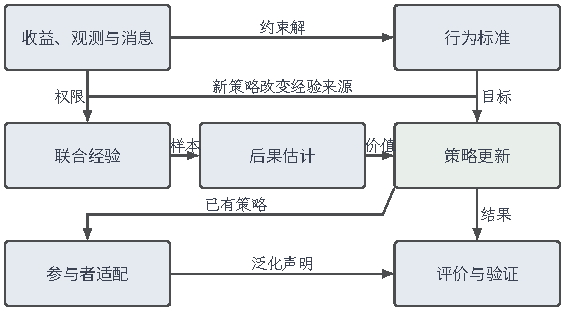
\includegraphics[width=95.652mm]{figures/07-reinforcement-learning/03-task-expansion-and-trustworthiness/tikz/rl-multi-agent-map.pdf}
  \caption{多智能体求解中的问题关系。实线连接约束、交互记录与后果估计的用途，外侧回路表示策略更新改变后续经验来源；底部的适配与评价检查行为标准在所声明参与者范围内是否成立。}
  \label{fig:rl-multi-agent-map}
\end{figure}

% Outline: 7.1
\section{收益、信息与参与者的共同设定}
\label{sec:rl-multi-agent-setting}

% Outline: 7.1.1
\subsection{用联合动作、转移与个体回报定义决策过程}
\label{sec:rl-multi-agent-process}

把通道截成一次“谁先通过”的竞争，可以得到一个确定性的教学任务。初态为两人都尚未通过的$s_{\text{入口}}$，另有“1先通过”“2先通过”和“碰撞”三个终止状态；两人都能观察当前状态，并读取自己的奖励。在入口，各人选择前进$F$或等待$W$。联合动作$(F,W)$使1先通过，两人的奖励依次为$(-1,-2)$；$(W,F)$使2先通过，奖励为$(-2,-1)$。$(F,F)$导致碰撞，双方各得$-4$并终止；$(W,W)$使系统留在入口，双方各得$-1$，下一步重新选择。三个终止状态都吸收，后续奖励为0。这里的数值是独立教学设定，不取自前几章的随机网格。

这个小任务把多人问题新增的依赖具体化：推动状态变化的是联合动作，每个人的奖励可以不同，观察权限也须逐人规定。一般环境还可能让奖励、后继观测和终止标记共同随机产生，因此需要一个联合生成模型。

\begin{definition}[多参与者序贯决策]
\label{def:rl-multi-agent-game}
给定正整数$m$、非空状态空间$S$、各人的非空行动空间$\mathsf A_i$与非空观测空间$\mathsf O_i$，均配备可测结构。设参与者集合为$\mathcal N=\{1,\ldots,m\}$，用$-i$表示除$i$之外的参与者，$\mathsf A_i(s)$为$i$在状态$s$中的非空合法动作集合，合法状态—联合动作对构成可测集合。各人动作组成$\bm a=(a_1,\ldots,a_m)\in\prod_i\mathsf A_i(s)$。以下各核与策略均可测，允许的合法策略集合非空。环境以从合法状态—联合动作对到$S\times\mathbb R^m\times\prod_i\mathsf O_i\times\{0,1\}$上概率测度的联合反馈核
\[
 K(\mathrm ds',\mathrm d\bm r,\mathrm d\bm o',\mathrm dd\mid s,\bm a)
\]
一次生成后继状态$s'$、个体奖励向量$\bm r=(r_1,\ldots,r_m)$、下一联合观测$\bm o'$及终止标记$d\in\{0,1\}$。共同转移核和期望奖励分别是这一联合律的边缘与条件均值：
\[
 \begin{aligned}
 T(B\mid s,\bm a)
 &=K\!\left(B\times\mathbb R^m\times\prod_i\mathsf O_i
              \times\{0,1\}\mid s,\bm a\right),\\
 R_i(s,\bm a)
 &=\int r_i\,K(\mathrm ds',\mathrm d\bm r,\mathrm d\bm o',\mathrm dd\mid s,\bm a).
 \end{aligned}
\]
其中$B$是$S$的可测子集，并要求各合法$(s,\bm a)$下$\int|r_i|\,\mathrm dK<\infty$。有限或可数空间中的积分按相应点质量求和。这里没有假设奖励、观测、后继状态和终止标记条件独立；若要使用因子化接口，须另行给出因子分解。

行动权限由局部历史$I_{i,t}$限定：它只包含$i$在动作$t$之前获准取得的观测、自身过去动作、可见奖励和已收到的消息。执行第$t$步联合动作后，联合反馈核先产生反馈，各人只能把协议允许其看见的部分写入$I_{i,t+1}$；策略产生的消息及其送达时刻另由通信协议规定。策略$\pi_i(a_i\mid I_i)$只依据该参与者获准取得的局部观测、消息和自身行动记录选择动作。记各人的策略合称为$\bm\pi$。初始分布$\mu_0$专指物理初态分布；下式的期望还固定初始观测、初始消息与公共信号的生成约定。要求每个参与者的折扣奖励和绝对可积，即$\mathbb E\sum_{t\geq0}\gamma^t|r_{i,t}|<\infty$；有界逐步奖励是充分条件。参与者$i$要评价的未归一化折扣回报为
\[
 J_i(\bm\pi)=\mathbb E_{\mu_0,\bm\pi}
 \left[\sum_{t=0}^{\infty}\gamma^t r_{i,t}\right],
 \qquad 0\leq\gamma<1.
\]
\end{definition}

把所有人的策略合在一起称为联合策略$\bm\pi$。它能不能写成各人策略的乘积，取决于动作是怎样产生的：给定联合历史$\bm I$后，若各人独立地各自随机化，才有$\bm\pi(\bm a\mid\bm I)=\prod_i\pi_i(a_i\mid I_i)$；若行动前先广播过一个公共随机信号$c$（比如抽签决定谁先走），那么这种独立性只能在给定$c$之后使用。把信号平均掉，得到$\sum_c p(c\mid\bm I)\prod_i\pi_i(a_i\mid I_i,c)$，一般不能再拆成各自边缘分布的乘积。若所有人都只行动一次，可以把每组联合动作的收益排成一张矩阵，得到矩阵博弈：每个格子对应一个联合动作，格子里写各方收益。加入共同状态和转移后，就相当于“在每个状态上各摆一局矩阵博弈，而这一局的动作结果又决定下一局发生在哪个状态”，这称为随机博弈（stochastic game），Shapley 建立了其完全可观测形式的经典理论\scite{rl1-shapley1953-games}。

一个自然的简化念头：既然真正要优化的只是我自己的策略，能不能把其余人也当成“环境”的一部分，继续套用单人 MDP？答案是有条件的——当其他人都使用固定的状态条件策略、并且给定$s$后他们的联合动作与我的动作独立随机化时，可以把他们各种动作出现的概率当作随机转移的一部分，按概率把转移与奖励加权平均掉。这一步边缘化给出$i$实际面对的过程：
\begin{align}
 T_i^{\bm\pi_{-i}}(s'\mid s,a_i)
 &=\sum_{\bm a_{-i}}\bm\pi_{-i}(\bm a_{-i}\mid s)
 T(s'\mid s,a_i,\bm a_{-i}),\label{eq:rl-multi-agent-induced}\\
 R_i^{\bm\pi_{-i}}(s,a_i)
 &=\sum_{\bm a_{-i}}\bm\pi_{-i}(\bm a_{-i}\mid s)
 R_i(s,a_i,\bm a_{-i}).\nonumber
\end{align}
在通道中，对方以概率$q$等待时，自己前进的通过概率为$q$，期望即时收益为$q(-1)+(1-q)(-4)=-4+3q$。若对方学习后把$q$从$0.8$降到$0.2$，这两个量都会改变，尽管共同的$T$和$R_i$没有变化。因而，对$i$而言过程不再平稳，可能仅仅是因为边缘化时使用的对方策略变了，而非物理环境发生漂移。

使用式\eqref{eq:rl-multi-agent-induced}时，要检查的是$\mathbb P(\bm a_{-i}\mid s,a_i)=\bm\pi_{-i}(\bm a_{-i}\mid s)$，而不是要求其他人彼此独立。公共信号若使双方动作相关，观察到自身动作也可能改变对其他动作的判断，不能直接用其边缘分布加权；应先把信号纳入条件，再检查等式。另一个限制来自记忆：对方若按过去碰撞次数调整让行概率，当前位置就不足以预测其下一动作。需要把相关记忆或类型纳入充分状态，或者在历史上定义过程，才能讨论相应的评价与收敛；原有平稳MDP结论不能直接沿用。

% Outline: 7.1.2
\subsection{不同收益关系下的合作、零和与一般和问题}
\label{sec:rl-multi-agent-payoffs}

保留入口和两种动作，改变奖励就会改变要解决的问题。若两人共享奖励，可另设碰撞$-2$、都等待$-1$、恰好一人前进$2$，目标是共同避免冲突并尽快通行。若只比较谁先通过，可让$(F,W)$给第一人$1$，$(W,F)$给第一人$-1$，其余为$0$，第二人取相反收益。若各人承担自己的时间成本，则等待者可能比先行者损失更多，而碰撞同时损害双方。以上是分别说明三种收益关系的教学设定，不是同一奖励表。

这三种奖励安排恰好对应多智能体中三类典型的收益关系，也是后面判断“策略是否变好”的三种不同标准。\term{完全合作}（fully cooperative）意味着所有人评价的是同一个回报目标，相当于同一支队伍：把蛋糕做大对每个人都有利。\term{两人零和}（two-player zero-sum）要求每个结果满足$r_{1,t}+r_{2,t}=0$，即一方的每一分收益恰好是另一方的损失；对整条轨迹求和取期望便有$J_2=-J_1$，最典型的就是零和对抗。\term{一般和}（general-sum）则不限制各收益之间的关系，可以同时含有共同利益与个人冲突——通道里双方都不希望碰撞，却又都想先通过。还要特别强调：目标相同不代表两人能读到相同的观测与消息，更不保证两个各自独立学习的人能自发形成彼此兼容的让行约定。表\ref{tab:rl-multi-agent-payoffs}据收益关系列出对应的行为标准，使后续“改进”有明确的比较对象。

\begin{table}[htbp]
 \centering
 \begin{tabularx}{\linewidth}{@{}l >{\raggedright\arraybackslash}X >{\raggedright\arraybackslash}X@{}}
 \toprule
 收益关系 & 标准与单方偏离 & 额外社会选择\\
 \midrule
 完全合作 & 在允许的局部观测与消息条件下最大化共同$J$；单方改动也按共同收益计 & 若存在多个最优策略，仍需选择兼容约定\\
 两人零和 & 最大化最坏收益；偏离检验可被利用的程度 & 价值标准已给定，风险限制可另设\\
 一般和 & 各自偏离是否获利；可另优化福利 & 必须另定福利、公平及取舍\\
 \bottomrule
 \end{tabularx}
 \caption{同一任务接口在不同收益关系下的行为标准。完全合作可比较共同回报，零和可比较最坏收益，一般和须另行指定社会目标。}
 \label{tab:rl-multi-agent-payoffs}
\end{table}

一般和中，总收益与个人激励可能冲突。总收益很高的结果可能诱使一人立即偏离；没有人愿意单方偏离的结果也可能使双方收益都很低。奖励求和可以定义一种福利指标，却既不规定收益如何分配，也不保证个人愿意维持该结果。评价时必须把福利、分配和稳定性分别说明。

% Outline: 7.1.3
\subsection{不同行动、观测与通信时序下的信息结构}
\label{sec:rl-multi-agent-information}

收益关系确定之后，还要确定作出选择时知道什么。通道中的“我先走”若在对方行动前送达，可以支持本轮避让；若延迟一轮，只能进入$I_{i,t+1}$。图\ref{fig:rl-multi-agent-timing}为此分别标出观测、发信、收信、行动和反馈。训练日志事后收齐消息，不意味着动作$t$可以使用它。行动本身也有时序限制：顺序行动的后手可能观察先手动作，同时行动的双方则不能据本轮尚未提交的对方动作决策。

\Needspace{16\baselineskip}
实现时，依次调用程序不等于允许依次观察行动。PettingZoo以统一接口支持多类多智能体环境，其中智能体—环境循环（agent environment cycle, AEC）接口逐个调用参与者。用它实现同时行动任务时，仍要屏蔽本轮其他人尚未共同提交的动作，否则调用顺序就意外地让后手提前读到了本轮其他人的动作\scite{rl7-terry2021}

\begin{figure}[htbp]
 \centering
 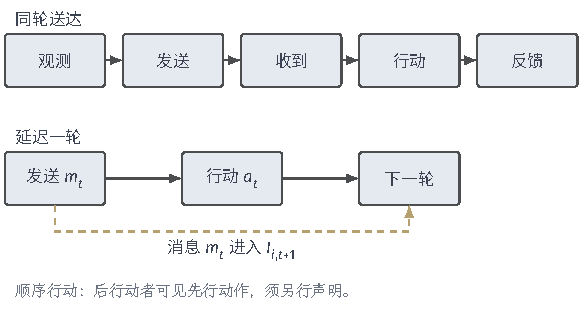
\includegraphics[width=98.616mm]{figures/07-reinforcement-learning/03-task-expansion-and-trustworthiness/tikz/rl-multi-agent-timing.pdf}
 \caption{消息何时进入策略输入。实线表示本轮可读取的观测与已送达消息，虚线表示下一轮才送达的消息；顺序行动还可能允许后手观察先行动作，这一权限不属于同时行动。}
 \label{fig:rl-multi-agent-timing}
\end{figure}

确定送达时刻后，还须规定消息携带什么。通信模型CommNet让参与者发送连续向量，把同伴发送的消息聚合成一个表示，再将其用于协作决策。这些表示能成为本轮策略输入的前提仍是动作前按协议送达，网络中的聚合运算不能替代实际通信权限\scite{rl7-sukhbaatar2016}

前面的讨论默认每个人都能看到完整状态，但真实场景往往不是这样：过道里看不到拐角后面是否有人，扑克玩家也看不到对手的底牌。于是需要给每个参与者单独规定他能看到的观测，而不是假设大家共享同一个$s$；各人看到不同信号的随机博弈称为\term{部分可观测随机博弈}（partially observable stochastic game, POSG）。把定义\ref{def:rl-multi-agent-game}中“下一观测”的条件单独取出，常将定义\ref{def:rl-multi-agent-game}中的观测条件边缘记为联合观测核$K_o(\bm o'\mid s',\bm a)$，并另给初始观测分布，说明状态怎样生成每个人看到的信号。采用这一简化接口，意味着观测边缘在给定$(s',\bm a)$后不再依赖旧状态；它不表示观测与奖励或终止反馈条件独立，完整耦合关系仍由$K$规定。局部观测$o_i$不等于完整状态$s$。若进一步共享团队奖励、并要求各策略只使用自己的历史，就得到\term{分散部分可观测马尔可夫决策过程}（decentralized POMDP, Dec-POMDP）：大家为同一个回报行动，却分别依据各自的观测、动作、奖励历史与合法消息作出选择。这里的困难超出单人 POMDP：即使把各人的观测合起来足以恢复状态，每个人在决策时也没有权限读取别人的观测。通信可以表示为动作的一部分或单独的消息阶段，顺序行动可以在状态中标记当前行动者；这些建模方式都必须保留实际观测范围和消息送达时序的限制\scite{rl7-bernstein2002}。

局部观测和可读行动历史对策略的限制可以用一个有限隐藏牌面游戏说明。这不是标准扑克；以下规则定义了全部随机性与收益。机会方以各$1/2$的概率给参与者1发高牌$H$或低牌$L$，只有1看见牌，两人先各投入一单位。1先选择下注$B$或过牌$K$：下注后由2选择弃牌$F$或跟注$C$；过牌后由2选择过牌$K$或下注$B$。若2也过牌，立即摊牌；若2下注，1再选弃牌$F$或跟注$C$，随后结束。摊牌时，高牌由1赢，低牌由2赢；无人加注时胜者净得$1$，跟注后胜者净得$2$。有人弃牌时，未弃牌者净得$1$。另一人取相反净收益，全局只有终局收益，不设折扣。

图\ref{fig:rl-multi-agent-card-tree}把这些规则展开成完整历史树：顶部机会节点生成牌面，圆节点表示决策，叶节点给出1的净收益。面对1首次下注，2不能区分高牌与低牌分支上的两个节点，因而它们属于同一\term{信息集}（information set），即依据该参与者已取得的观测、动作、奖励和消息无法区分的一组完整历史。2必须在两处使用相同的跟注概率；按牌面分别设概率就使用了参与者2并未看到的牌面。相反，2能够看见1是下注还是过牌，这两种情形必须属于不同的信息集。

\begin{figure}[htbp]
 \centering
 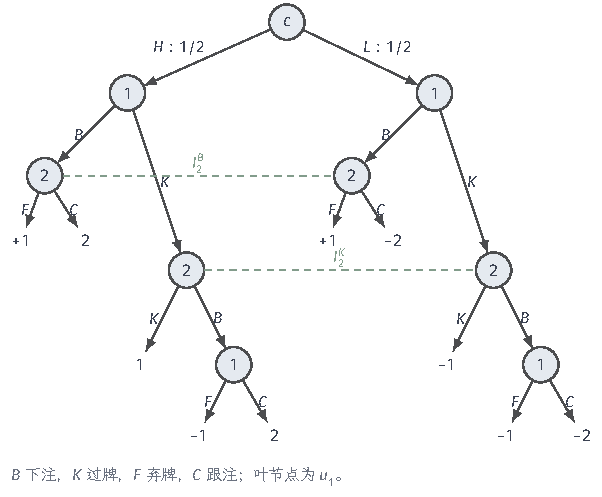
\includegraphics[width=101.946mm]{figures/07-reinforcement-learning/03-task-expansion-and-trustworthiness/tikz/rl-multi-agent-card-tree.pdf}
 \caption{隐藏牌面教学游戏的完整历史树。虚线各自连接2面对下注、面对过牌时不能区分的节点；1知道牌面，其节点不跨牌面合并。叶节点标1的净收益，2取相反数。}
 \label{fig:rl-multi-agent-card-tree}
\end{figure}

这里引入的\term{信息集}（information set），直观上就是“在某个参与者看来无法区分的一组完整局面”：处在同一信息集的节点，对他而言可能给出完全相同的观察和历史，所以他必须在这些节点上使用同一套动作概率。但信息集也不能抹掉参与者自己的记忆。\term{完全回忆}（perfect recall）要求同一信息集里的所有历史，都具有相同的“自己过去知道过什么、做过什么”序列。

% Outline: 7.1.4
\subsection{信息权限与联合策略表示}
\label{sec:rl-multi-agent-permissions}

若由一个能取得全局状态与各人历史的控制器选择联合动作，就可以集中决策。困难在于训练与部署可读取的变量不同：训练通常在仿真器或服务器上进行，可以记录全局状态、联合动作和各人的历史；真实部署时，每个人却只有局部传感器，不能即时读取其他人的位置、局部观测与历史，通信也可能受限。这些集中变量可以帮助训练评论家，但执行策略仍不能依赖部署时读不到的变量。\term{集中训练、分散执行}（centralized training with decentralized execution, CTDE）正是把这两种权限分开：训练时允许用全局状态、联合动作或其他人的历史来估计价值，行动策略在部署时则只能读取本地历史及获准送达的消息。

\begin{figure*}[htbp]
 \centering
 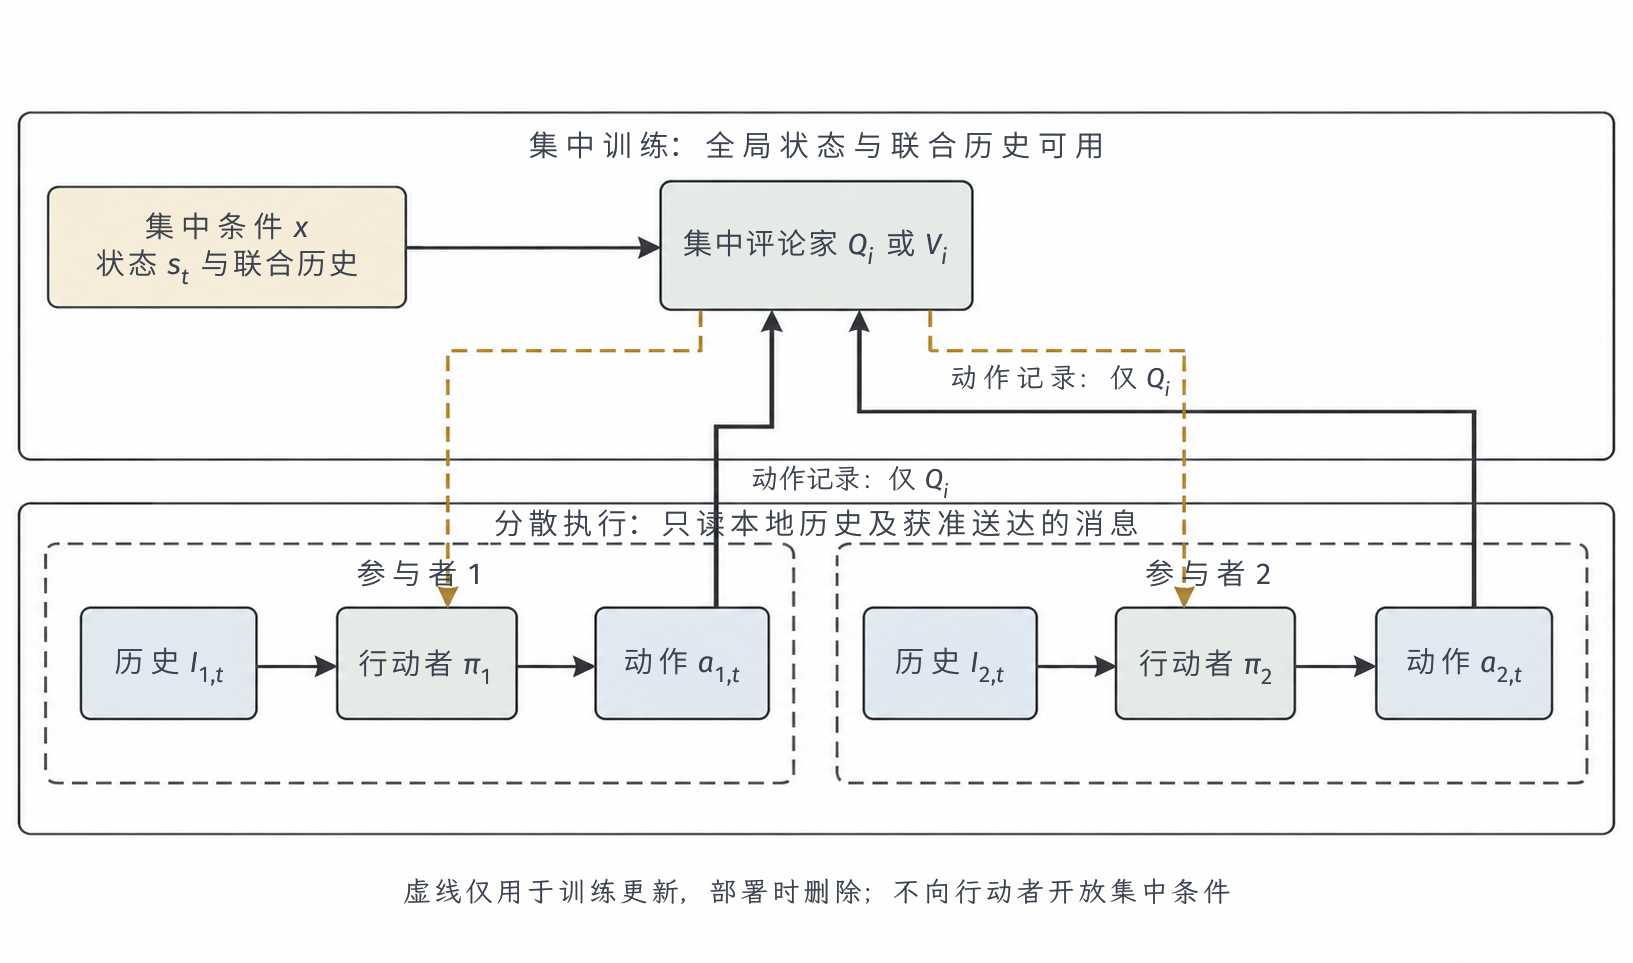
\includegraphics[width=157.400mm]{figures/07-reinforcement-learning/03-task-expansion-and-trustworthiness/generated/rl-multi-agent-ctde/figure.png}
 \caption{CTDE中的集中训练与分散执行。上区的集中评论家可使用全局状态及联合历史，下区各行动者只使用本地历史和获准消息。向评论家上送的当前动作仅用于$Q_i$，估计$V_i$时不取当前动作作为条件；部署时删除训练虚线，也不向行动者开放集中条件。两个参与者仅为示例。}
 \label{fig:rl-multi-agent-ctde}
\end{figure*}

在执行权限相同的前提下，还可以选择是否共享参数。若两人的观测、动作和角色含义兼容，共享$\pi_{\bm\theta}(a_i\mid I_i)$可让同一函数服务两人，但不会让他们读取对方的局部观测或消息。加入身份编码$e_i$后，网络可按编号形成“1先走、2等待”的约定；身份重排却可能使该约定失效。独立参数容纳不同动作接口或角色，但需分别存储和拟合各人的网络，并寻找能彼此配合的策略组合。参数量和训练样本需求还取决于网络结构与任务，不能仅由参数独立就断言样本成本更高。身份是否必要，应由任务中的角色含义决定。

通信也可以参与参数学习。可微智能体间学习（differentiable inter-agent learning, DIAL）在训练时通过可微信道传递梯度，使发送者得到关于消息用途的反馈，部署时则改用受限的离散消息。连续训练近似与实际离散信道并不相同，量化可能改变接收到的消息内容，因此仍要检查部署消息能否支持学到的协调行为\scite{rl7-foerster2016}

要检查这种训练与执行差异，协议必须说明谁向谁发送什么、何时送达，以及花费多少带宽。表\ref{tab:rl-multi-agent-communication}比较四种可与CTDE组合的接口。能否通过消息反向传播属于训练计算条件，链路延迟、带宽和接收权限则约束实际执行，两者不能相互替代。

\begin{table}[htbp]
 \centering
 \begin{tabularx}{\linewidth}{@{}l >{\raggedright\arraybackslash}X >{\raggedright\arraybackslash}X@{}}
 \toprule
 接口 & 发送者、接收者与内容 & 时序、带宽及训练／执行条件\\
 \midrule
 固定协议 & 每人向指定邻居发角色或让行码 & 动作前收信；固定比特数；两阶段协议均保持\\
 可微通信 & 所有人向聚合器或同伴发实向量 & 每轮一至多次交换；向量维数固定；执行须保留信道\\
 离散消息 & 每人向获准接收者发有限字母表符号 & 训练可用连续松弛；执行量化后重新核验\\
 图消息传递 & 节点向图邻居发嵌入或定向消息 & 边数与轮数决定带宽；部署只能使用可发现的边\\
 \bottomrule
 \end{tabularx}
 \caption{四种消息接口的执行条件。比较时须同时说明发送者与接收者、消息内容、送达时刻及通信成本，而不只报告训练中是否可微。}
 \label{tab:rl-multi-agent-communication}
\end{table}

若并非所有人都需要同一条消息，可以进一步学习发送对象。定向多智能体通信（targeted multi-agent communication, TarMAC）用定向寻址计算接收权重，让不同接收者聚合不同内容。它解决的是“消息给谁”，可以与消息内容的表示、训练信道的选择共同使用，但仍须符合部署的接收权限\scite{rl7-das2019}

% Outline: 7.1.5
\subsection{不同数据访问与参与者变化方式下的学习问题}
\label{sec:rl-multi-agent-access}

相同的两人通道，还会因交互记录的采集、访问权限和对方变化方式而形成不同学习问题。对方遵守固定避让规则时，学习者可以探索其响应；双方共同训练时，刚估计的规则下一轮可能已改变；从历史策略库抽样时，每场经验还取决于抽到了哪个版本。表\ref{tab:rl-multi-agent-access}将参与者条件与记录访问权限交叉列出。其中“可改变”只指学习者按协议能控制的因素，第三方主动改变策略不属于学习者的采集权限。

\begin{table}[htbp]
 \centering
 \begin{tabularx}{\linewidth}{@{}l >{\raggedright\arraybackslash}X >{\raggedright\arraybackslash}X >{\raggedright\arraybackslash}X@{}}
 \toprule
 参与者条件 & 在线访问 & 固定联合日志 & 有限批次访问\\
 \midrule
 固定伙伴 & 可改自身行为，伙伴不变 & 不可重采；还原固定版本 & 批间改自身，批内固定\\
 同步学习者 & 可按约定更新双方 & 仅观察历史更新，不能重放新响应 & 批间同步更新，批内冻结\\
 群体抽样 & 可改获准的抽样分布 & 只能使用已记录群体支持 & 批间改抽样，批内固定\\
 主动适应者 & 自身动作可诱发其响应，未必可控 & 响应机制可能不可识别 & 须声明对方是否随批内历史更新\\
 \bottomrule
 \end{tabularx}
 \caption{记录访问权限和参与者变化共同限定可做的采集。有限批次若包含对方的批内适应，整批就不能被描述为固定联合策略产生的交互记录。}
 \label{tab:rl-multi-agent-access}
\end{table}

多智能体建模不要求所有参与者都在学习：即使只优化一个策略，也须表示其他行为怎样共同决定结果。反过来，同时运行多个固定规则代理或多个语言模型角色，并不能说明发生了强化学习。还需给出被优化的策略、交互产生的反馈和更新所针对的回报。“多人对话”描述的是交互形式，不能代替这些学习条件。

% Outline: 7.2
\section{不同收益关系下的行为标准}
\label{sec:rl-multi-agent-solutions}

模型建好了，但“回报提高”在不同收益关系下含义完全不同：合作时是共同蛋糕变大，零和时是最坏情况下不吃亏，一般和时则要问有没有人愿意单方面改变行为。因此在讨论学习之前，必须先选定衡量行为的标准。下面保留有限两动作的教学接口，分别考察共同目标下的团队最优、零和对抗中的最坏情形价值、以及一般和博弈中的单方偏离稳定性。三者对应的收益关系不同，不能把其中一种意义上的“改进”当成另一种标准也得到了满足。

% Outline: 7.2.1
\subsection{共同目标下的联合最优标准}
\label{sec:rl-multi-agent-team}

共享回报时，目标函数很直接：最大化共同的$J(\bm\pi)$。但这里有一个初学者极易忽略的限制——可搜索的策略范围只能是部署时真正可执行的$\Pi_{\text{分散}}$，其中每条策略都必须满足局部观测范围、消息时序和公共随机性的约束。训练服务器可以用全局状态或联合历史来帮助估计、帮助求解，却不能因此让部署时的行动者直接读到这些变量。一个能看到全局的“中央大脑”当然可能做得更好，下面的包含关系就给出这种集中求解相对分散最优值的上界。

\begin{theorem}[集中与分散策略的可行集合]
\label{thm:rl-multi-agent-inclusion}
设奖励有界且$0\leq\gamma<1$。若集中控制器在每个决策时刻取得分散系统的全部可用历史，还能模拟其私有随机性、公共随机性和合法通信，就能为每个分散策略生成相同的轨迹分布。按所实现的分布识别策略，有
\[
 \Pi_{\text{分散}}\subseteq\Pi_{\text{集中}},
 \qquad
 \sup_{\bm\pi\in\Pi_{\text{分散}}}J(\bm\pi)
 \leq
 \sup_{\pi\in\Pi_{\text{集中}}}J(\pi).
\]
\end{theorem}
\begin{proof}
对任意分散策略$\bm\pi$，让集中控制器分别保存各人的局部历史，并在每一时刻按原协议产生公共信号、私有随机数和消息，再调用各$\pi_i$生成联合动作。这样既不改变随机机制，也不向局部策略额外提供其他人的观测或消息。模拟从相同的初始历史分布开始；若直到$t$的联合历史分布相同，相同策略调用就产生相同的条件动作分布，未变的联合反馈核和合法消息生成、送达协议继而产生相同的$t+1$历史分布。这里的反馈包括各人可见的奖励、观测与终止标记，不能只比较状态边缘。归纳可得所有有限轨迹分布一致。有界奖励与$\gamma<1$保证相应折扣回报期望一致，所以每个分散系统可达的回报都能由集中控制器实现。对两种可达集合取上确界，便得到不等式；若有限问题中最优策略存在，上确界可写成最大值。
\end{proof}

集中上界不一定能分散实现。设通行前产生均匀二值信号$c\in\{0,1\}$，两个值的概率各为$1/2$，只有两人都选$c$时团队得$1$，否则得$0$。集中控制器看到$c$，每次都能得$1$。对分散双方，假设各自观测均与$c$独立，不许互传观测，使用的随机数也独立于$c$及双方观测。允许公共随机数只能帮助两人协调，不能让任一人知道$c$；其动作仍与$c$独立。成功事件包含在第一人选对的事件中，故
\[
 \mathbb P(a_1=a_2=c)\leq\mathbb P(a_1=c)=\frac12.
\]
这里仅使用每个人动作与$c$的独立性，没有把逐个独立扩大为联合观测或联合动作的独立性。固定都选0可以达到$1/2$这一上界。若允许在行动前广播$c$，局部策略才有条件按信号选择，分散最优值也才恢复为1。

因此，声称团队最优时须同时给出回报目标和允许的观测、历史与消息条件。一次成功协调仅说明找到了一个有效行为，参数空间的局部最优也不等于整个可行策略集合的最优。若原问题的个人收益不同，更不能在没有另定目标的情况下把它改写成团队最大化。

% Outline: 7.2.2
\subsection{零和对抗下的极小极大标准}
\label{sec:rl-multi-agent-minimax}

先从直觉理解为什么在零和对抗中，确定性动作往往不可取、必须随机化。用一个“猜对方选哪侧”的两动作任务说明。
\begin{equation}
 \bm A=
 \begin{pmatrix}1&-1\\-1&1\end{pmatrix}.
 \label{eq:rl-multi-agent-matching}
\end{equation}
第一人固定选任一侧，第二人总能选一列使其收益为$-1$；第一人均匀随机时，两列的期望却都为0。因而随机化的用途是抵御对手对行动偏好的利用，而不是减少单条轨迹的不确定性。

把这个例子推广。对一般收益矩阵$\bm A\in\mathbb R^{p\times q}$，令$\bm x\in\Delta_p$、$\bm y\in\Delta_q$分别为两人在纯动作上的概率分布，这样的随机化称为\term{混合策略}（mixed strategy）；其中$\Delta_p$表示所有分量非负且总和为 1 的$p$维概率向量，$\Delta_q$同理。按行、列概率给各格收益加权，得到$\bm x^\top\bm A\bm y$，由第一人最大化、第二人最小化。固定对方策略后，自身的最优选择称为\term{最佳响应}（best response）；若两人都固定对方策略、谁也无法再通过单方面改变来提高收益，这样的组合就称为\term{鞍点}（saddle point）——在收益曲面上，沿一方方向是极大、沿另一方方向是极小，形如马鞍。要抵御对手利用自己的偏好，第一人不能只针对某个平均对手拿高分，而必须保证在所有允许的对手策略下都能守住一个收益下界。于是有两种设想博弈顺序：第一人先公开自己的混合策略、第二人随后针对它最小化，第一人在这个前提下取最大化；或者反过来。直观上“先承诺、后被针对”似乎吃亏，但在有限动作且双方都允许任意混合策略的条件下，两种顺序恰好给出同一个博弈值。

对正整数$p,q$及收益矩阵$\bm A\in\mathbb R^{p\times q}$，若双方允许全部行、列混合策略$\Delta_p,\Delta_q$，收益$\bm x^\top\bm A\bm y$对双方策略双线性，则有限零和极小极大结论给出
\[
 \max_{\bm x\in\Delta_p}\min_{\bm y\in\Delta_q}\bm x^\top\bm A\bm y
 =\min_{\bm y\in\Delta_q}\max_{\bm x\in\Delta_p}\bm x^\top\bm A\bm y.
\]
双方的最优混合策略都存在，组成鞍点。
这个结论把有限双线性零和问题的两种优化次序接成同一个博弈值。它让后继状态上的矩阵收益得到确定的最坏情形价值，供控制备份调用；并未说明有限样本或神经网络更新能求出这一价值。有限矩阵博弈、相关建议、遗憾与平均策略的一般分析可参考\BookChapterRef{chap:game-theory-and-multi-agent-decision}{卷2《数学准备：概率、因果与决策》“多方策略的响应与演化”章}。允许全部混合策略是关键条件；把策略限制为非凸神经网络参数类后，允许集合已经改变，不能直接沿用等式。

上述阶段博弈值可以直接嵌入多步决策。对完全可观测的两人零和折扣随机博弈，把$Q(s,\cdot,\cdot)$看成状态$s$上的一张收益矩阵，用$\operatorname{val}Q(s)$表示它的极小极大值。即时奖励之后，双方在后继状态仍按最坏情形标准选择，于是控制备份就是把单人备份里的“对动作取最大”换成“对联合矩阵取极小极大值”：
\begin{equation}
 (\mathcal B Q)(s,\bm a)
 =R_1(s,\bm a)+\gamma\sum_{s'}T(s'\mid s,\bm a)
           \operatorname{val}Q(s').
 \label{eq:rl-multi-agent-minimax-backup}
\end{equation}
极小极大Q学习（Minimax-Q）用一次采样中的$r_{1,t}+\gamma\operatorname{val}Q(s_{t+1})$替代转移期望，再按步长$\alpha_t$更新当前表项。若奖励为1、后继博弈价值为0，旧值0.4以步长0.5向目标1移动，得到0.7。与单智能体只取动作最大值不同，每个后继价值都需要求解阶段线性规划；这一运算使Minimax-Q的备份反映对手的最坏响应\scite{rl7-littman1994}

这给出了目标的计算依据，还没有给出任意实现的收敛保证。表格分析另需有界奖励、各状态联合动作充分访问、合适的随机逼近步长和正确的阶段价值求解。深度逼近改变估计误差，局部观测改变状态条件，共同学习又可能改变状态与联合动作的访问覆盖；这些情形都需单独分析。

% Outline: 7.2.3
\subsection{一般和博弈下的均衡与社会目标}
\label{sec:rl-multi-agent-equilibria}

双方收益并不严格相反时，一个稳定性问题是：给定其他人都不变，我单方面换成别的策略能不能获益？例如两人各选左$L$或右$R$作为让行约定，同选一侧时双方各得2，选不同侧时双方各得0。这是一次行动后即终止的协调博弈，收益表为
\[
 \begin{array}{c|cc}
       &L&R\\ \hline
 L&(2,2)&(0,0)\\
 R&(0,0)&(2,2)
 \end{array}.
\]
若双方都选左，任一人单独改选右就会把自己的收益从2降到0；双方都选右也一样。稳定性在此检查的是单方改变，不要求两个稳定约定中必须选出唯一一个。

一般地，给定正整数$m$、各人的非空有限动作集$\mathsf A_i$及收益函数$u_i:\prod_j\mathsf A_j\to\mathbb R$。各人独立选择混合策略$\pi_i\in\Delta(\mathsf A_i)$，联合分布为$\bm\pi=\prod_i\pi_i$。若对每个参与者$i$和每个替代混合策略$\pi_i'\in\Delta(\mathsf A_i)$都有
\[
 \mathbb E_{\bm\pi}[u_i(\bm a)]
 \geq \mathbb E_{\pi_i'\prod_{j\ne i}\pi_j}[u_i(\bm a)],
\]
就称$\bm\pi$为\term{Nash均衡}（Nash equilibrium）。它将“其他人不变”写成固定$\bm\pi_{-i}$，将“任何单方改变都无利可图”写成对全部$\pi_i'$的不等式。在上述协调博弈中，都左与都右都是纯策略Nash均衡。
若由联合分布$q(\bm a)$产生动作建议，\term{粗相关均衡}（coarse correlated equilibrium, CCE）要求在看到建议之前改用固定动作也不能获利：
\[
 \mathbb E_q[u_i(\bm a)-u_i(b_i,\bm a_{-i})]\geq0
 \quad\text{对所有 }i,b_i.
\]
\term{相关均衡}（correlated equilibrium, CE）进一步允许根据收到的自身建议选择替代动作，要求
\[
 \sum_{\bm a_{-i}}q(a_i,\bm a_{-i})
 [u_i(a_i,\bm a_{-i})-u_i(b_i,\bm a_{-i})]\geq0
 \quad\text{对所有 }i,a_i,b_i.
\]

两个建议标准的区别在于偏离决定的时刻：CCE只比较事前选定的固定动作，CE还比较收到某个建议之后的替换，故CE约束更强。定义中的CE式没有除以建议概率，罕见建议带来的收益差仍按发生概率计权。Nash限定独立随机化，CE与CCE则允许联合建议相关。在上述协调博弈中，以各$1/2$概率建议双方都左或都右可以形成CE；将其边缘化后再独立抽样，却有一半概率失配。联合分布中的相关建议因此是行为标准的一部分。

当前两动作协调例说明联合建议怎样避免失配，还不能展示CE与CCE的严格差别。每位参与者都只有两个动作时，换成某个固定动作的CCE约束已经包含唯一的非平凡建议替换。下面增加第三个动作，才把两种偏离权限分开。

\begin{example}[事前固定偏离与收到建议后的偏离]
  \label{ex:rl-multi-agent-ce-cce}
  参与者1有动作$A,B,C$，参与者2有动作$L,R$。参与者1的收益为
  \[
    \begin{array}{c|rr}
          &L&R\\ \hline
      A& 0&-1\\
      B&-1& 0\\
      C& 1&-1
    \end{array},
  \]
  参与者2的收益恒为0。联合建议以各$1/2$概率给出$(A,L)$或$(B,R)$，照做时参与者1的期望收益为0。如果事前固定改选$A,B,C$，期望收益分别为$-1/2,-1/2,0$，都不能提高收益；参与者2也没有获利偏离，因此该建议分布满足CCE。

  但参与者1收到建议$A$时，已知道对方收到$L$。此时从$A$改为$C$会把收益从0提高到1，违反CE约束。这一偏离的未条件化期望获利为$1/2$，也直接违反定义中的CE不等式。因而CCE允许的分布可以被CE排除，原因是偏离者能否利用已经收到的建议。
\end{example}

有限个参与者、各人非空有限纯动作集且允许全部混合策略时，至少存在一个混合Nash均衡；这一存在性结论用于确认上述行为标准并非空要求。它并未保证高效计算，也未保证任意学习过程都会收敛到均衡\scite{rl7-nash1950}

表\ref{tab:rl-multi-agent-equilibria}比较这些标准的偏离对象。用于多步问题时，偏离者可能同时改变后续行为，因此“替代动作”须扩展为从全部相关历史到动作的\emph{完整策略}；若只检查受限的状态条件偏离，也须明确这一限制。即使某个已访问状态满足阶段CE，后续策略改变仍可能提高整个轨迹的回报，不能据此宣称序贯稳定。

\begin{table}[htbp]
 \centering
 \begin{tabularx}{\linewidth}{@{}l >{\raggedright\arraybackslash}X >{\raggedright\arraybackslash}X@{}}
 \toprule
 标准 & 偏离对象与信号 & 保证与未规定部分\\
 \midrule
 Nash & 固定对手后换自身策略；独立随机化 & 无单方收益改进；未最大化福利\\
 CE & 根据自己收到的建议换动作 & 无建议条件偏离；需合法相关信号\\
 CCE & 看建议前改为固定动作 & 无事前固定偏离；不排除条件偏离\\
 福利目标 & 按给定聚合函数选联合结果 & 可比较社会收益；不自动保证稳定或公平\\
 \bottomrule
 \end{tabularx}
 \caption{行为标准所检查的偏离与留下的选择。表中动作条件针对固定阶段博弈；用于序贯问题时，需要声明完整策略偏离还是某个受限偏离类。}
 \label{tab:rl-multi-agent-equilibria}
\end{table}

Nash Q学习（Nash Q-learning, Nash-Q）将阶段Nash标准用于多步目标：在后继状态的各人价值矩阵中选取均衡$\bm\sigma^*(s')$，按该均衡的联合动作概率加权各人的后继价值，得到
\[
 y_i=r_i+\gamma\sum_{\bm a'}\bm\sigma^*(\bm a'\mid s')
                         Q_i(s',\bm a').
\]
例如，在后继协调矩阵中选“都左”，各人后继值均为2；即时奖励0、$\gamma=0.9$时，目标就是1.8。若多个阶段均衡给出不同收益，目标将依赖选取规则；规则的不连续还可能改变更新动态。Nash-Q原文的收敛分析要求特殊的阶段均衡条件，存在性本身不能支持一般深度Nash-Q的收敛声明\scite{rl7-hu2003}

% Outline: 7.3
\section{多智能体的联合经验获取}
\label{sec:rl-multi-agent-data}

行为标准定下来之后，紧接着的问题是：要用什么样的联合交互记录才能估计它？多智能体在这里有一个单人问题没有的特殊困难——每个人都试过自己的动作，并不等于“团队”试过所需的动作组合。在通道里，两个人各自都单独前进过很多次，但“恰好一人前进、一人等待”这种关键组合可能从未同时出现。因此采集方案不能只规定每人探索什么，而要从待估量出发，规定参与者、行动前可读的历史和他们实际采取的联合行为，再回头检查这批记录能支持什么结论。若只有一份固定日志，则整个过程要从还原它的生成条件开始，不能假设还能重新采集。

% Outline: 7.3.1
\subsection{联合经验需求与采集方案的确定}
\label{sec:rl-multi-agent-collection-plan}

评价现有让行团队，需要部署伙伴分布下的当前策略回报；寻找自身改进，需要比较候选行为；检验单方偏离，还需要候选完整策略可能到达的后续状态。即使轨迹数量相同，对这三个任务也可能提供截然不同的支持。表\ref{tab:rl-multi-agent-data-needs}据此列出联合行为需求与可以控制的采集因素。

\begin{table}[htbp]
 \centering
 \begin{tabularx}{\linewidth}{@{}l >{\raggedright\arraybackslash}X >{\raggedright\arraybackslash}X@{}}
 \toprule
 待估量 & 所需联合行为与参与者范围 & 可控因素与预算\\
 \midrule
 当前团队回报 & 当前联合策略及部署伙伴分布 & 固定策略，重复独立回合，预算按回合计\\
 自身改进价值 & 固定或条件化伙伴下的候选自身动作 & 探索强度与起点；按联合环境步计\\
 单方偏离收益 & 原对手固定，完整候选响应的轨迹 & 响应训练、验证分开；计对手查询\\
 新伙伴协调 & 留出伙伴及允许探测的历史 & 伙伴抽样、角色与通信；计适应步数\\
 \bottomrule
 \end{tabularx}
 \caption{各待估量对应的采集需求。轨迹总数不能代替所需联合行为的覆盖，预算还应列明向各类参与者分配的数量。}
 \label{tab:rl-multi-agent-data-needs}
\end{table}

执行采集前，应给出伙伴或群体分布$q(k)$、各行为策略$\beta_i^{(k)}$、角色分配、行动时序和探索噪声。记录中要区分参与者身份、参数版本及本回合是否继续更新，才能分清是谁以哪套规则产生经验。均匀抽样可以扩大预期支持，却不能保证有限样本中已出现罕见联合事件。若固定日志缺少来源，只能保留可知条件；轨迹呈现的频率不足以还原当时的行为概率。

\Needspace{24\baselineskip}
按版本组织经验的一个实例是OpenAI Five。其报告中，训练对局的80\%面向最新参数，20\%面向历史版本，历史版本的抽样分布还随对局表现调整。这说明保存历史对手本身不能还原来源组成，还须保存采样时的版本分布\scite{rl7-berner2019}

% Outline: 7.3.2
\subsection{联合轨迹采集与生成条件记录}
\label{sec:rl-multi-agent-records}

采集时，用于一步更新的联合记录至少应让当前与后继采用同一组评论家条件变量：状态评论家保存$(s_t,\bm a_t,\bm r_t,s_{t+1},d_t)$；基于联合观测或历史的评论家则保存$(\bm o_t,\bm a_t,\bm r_t,\bm o_{t+1},d_t)$，并关联轨迹顺序、回合边界，以及足以按顺序重建后继历史的消息收发、可见奖励与反馈字段。这里$d_t$是联合反馈核中的终止标记。若评论家条件还含其他集中变量，也须同时保存其当前值和后继值，不能用$\bm o_{t+1}$默认替代$s_{t+1}$。记录还要关联各人身份、策略版本和合法动作集合。离策略校正需要伙伴抽样概率，以及给定真实可用历史后的动作概率；若动作相关，还要记录公共信号或相关采样机制。版本号仅能指向参数，不能独自确定实际概率，因此还须保留参数检查点、探索噪声规则和动作屏蔽逻辑。

多人联合探索可以由一个按钮任务看清：只有双方在同一步都按按钮，协作事件才发生。若两人独立地各以0.1的概率按，事件概率为$0.1^2=0.01$。若动作前向两人广播同一个$c\sim\operatorname{Bernoulli}(0.1)$，并约定$c=1$时两人都按、$c=0$时两人都不按，则每人的按键边缘概率仍为0.1，双方同按的概率却变为0.1。变化来自共同随机性引起的动作相关，并非各人的按键次数增加。图\ref{fig:rl-multi-agent-exploration}还列出角色条件和通信这两种协调依据；每种依据都须在动作之前实际送达。

\begin{figure}[htbp]
 \centering
 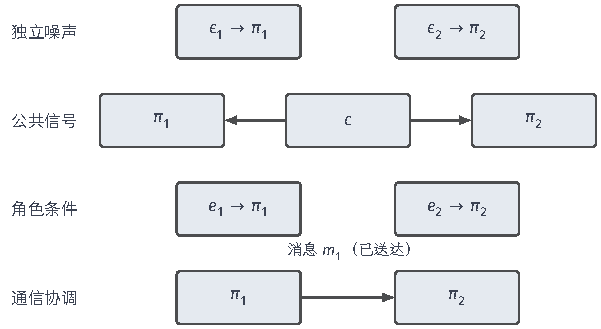
\includegraphics[width=101.741mm]{figures/07-reinforcement-learning/03-task-expansion-and-trustworthiness/tikz/rl-multi-agent-exploration.pdf}
 \caption{联合探索的四种动作与消息生成路径。独立噪声不能保证共同事件发生；公共信号、角色条件和通信分别提供协调依据，箭头表示执行者在动作前实际取得的观测、消息或随机信号。}
 \label{fig:rl-multi-agent-exploration}
\end{figure}

在公共信号例中，真实联合概率$\mathbb P(a_1=\text{按},a_2=\text{按})=0.1$，边缘概率的乘积却是0.01。若将后者作为行为概率，重要性权重就会错十倍。动作依赖通信或同一随机数时也须作同样检查：可以直接保存真实联合概率，也可以先保存使条件独立成立的信号，再计算条件概率的乘积。

% Outline: 7.3.3
\subsection{经验分布变化与目标覆盖检验}
\label{sec:rl-multi-agent-coverage}

取得联合交互记录后，先检查其生成策略、伙伴组成和采集协议是否仍适用于目标。由式\eqref{eq:rl-multi-agent-induced}，版本$k$的对手以$q^{(k)}$概率等待时，自身前进的诱导奖励为$-4+3q^{(k)}$。等待概率改变$\Delta q$，奖励就改变$3\Delta q$，后续状态占用也可能随通过概率变化。不过，版本号变化只是潜在漂移的线索；是否实际发生漂移，应结合分层统计、预测残差或已知策略概率判断。

随后要检查支持，即生成机制是否可能产生目标需要的事件。设日志只以各$1/2$概率生成$(0,0)$和$(1,1)$，非对角联合动作概率为0。每个人的两个动作都出现了，但$(0,1)$和$(1,0)$仍无支持。若两个奖励模型在对角线上都给0，在非对角线上却分别给$10$和$-10$，它们产生的日志分布完全相同，对候选偏离的预测却相反。这个反例表明：没有额外结构假设，边缘覆盖不足以识别未见的联合效果。

表\ref{tab:rl-multi-agent-support}按待估量列出需要检查的支持。实践中还须区分总体概率和样本频率：有限样本未出现某事件，不足以证明其总体概率为零，应连同频率报告不确定性。同样，未检出漂移也不足以证明生成机制恒定。

\begin{table}[htbp]
 \centering
 \begin{tabularx}{\linewidth}{@{}l >{\raggedright\arraybackslash}X >{\raggedright\arraybackslash}X@{}}
 \toprule
 估计对象 & 所需支持 & 典型缺失\\
 \midrule
 目标联合价值 & 目标到达状态及联合动作，目标伙伴 & 某种配合从未采到\\
 最佳响应 & 固定对手下候选完整策略的状态与动作 & 只记录原策略的到达状态\\
 个体反事实优势 & 固定其他动作后的自身候选动作 & 仅含对角动作的记录不能估非对角值\\
 消息条件价值 & 对应消息历史、角色、策略类型 & 未记消息使条件分布不可恢复\\
 \bottomrule
 \end{tabularx}
 \caption{待估量所需的联合支持及常见缺口。增加集中状态输入可以细化条件，却不能提供未发生的联合行为后果。}
 \label{tab:rl-multi-agent-support}
\end{table}

% Outline: 7.3.4
\subsection{覆盖充分时的可用经验构造}
\label{sec:rl-multi-agent-reweight}

目标事件有支持之后，还要处理来源比例与目标不一致的问题。只用最近窗口可缩小版本跨度，代价是丢弃旧版本策略产生的交互记录；按参与者分层可控制伙伴组成；将类型或版本输入价值网络，可分别估计不同对手条件下的后果。若已知生成概率，还可以用重要性校正把行为分布下的期望换为目标分布下的期望。这些措施分别改变样本选择、估计条件或期望测度，可以组合，但没有一种能无条件消除共同学习的非平稳性。

令$k$为一回合抽到的策略群体身份，$\tau$为长度$H$的完整理论轨迹，$q_\beta,q_\pi$分别为行为与目标的伙伴分布。要换算期望，先假设两过程具有相同的初始分布、联合反馈核$K$、环境终止规则和消息送达协议，并且目标联合轨迹分布对行为分布绝对连续，即目标有概率的事件在行为中也有概率。下面的$p_\pi,p_\beta$是相应完整轨迹律的质量函数或共同支配测度下的密度。将轨迹生成概率相除，得到
\begin{equation}
 w(\tau,k)=\frac{p_\pi(\tau,k)}{p_\beta(\tau,k)}
 =\frac{q_\pi(k)}{q_\beta(k)}
   \prod_{t=0}^{H-1}
   \frac{\bm\pi(\bm a_t\mid\bm I_t,k)}
        {\bm\beta(\bm a_t\mid\bm I_t,k)}.
 \label{eq:rl-multi-agent-is}
\end{equation}
两过程相同的联合反馈核项在比值中整体相消；这一步不要求后继状态、奖励、观测与终止反馈在核内独立。留下的是伙伴抽样与逐时刻联合动作的概率比。策略产生的消息若未包含在动作内，还须保留消息概率比；公共信号分布若改变，也须乘上其比值。只有给定记录历史与公共信号后各人条件独立，联合动作比才能分解为$\prod_i\pi_i(a_{i,t}\mid I_{i,t},k)/\beta_i(a_{i,t}\mid I_{i,t},k)$。据此，对完整轨迹函数$f$有$\mathbb E_\pi f=\mathbb E_\beta[wf]$；只估计某个时刻的奖励时，逐决策形式使用截至该奖励的前缀比，不必包含未来动作。

把该权重用于可见记录时，还须能从记录恢复计算概率比所需的动作历史、伙伴身份和消息字段。若$f$与$w$均可由记录计算，完整轨迹上的换测度等式也给出记录上的相应等式；丢弃这些必要字段后，应先边缘化得到记录密度比，不能直接沿用完整轨迹的乘积。

实际构造可以按来源分层取样，恢复真实条件概率，再以所得权重加权回报或损失。按上述个体条件分解计算时，长度$H$的轨迹需要计算$mH$个个体策略概率，还包括伙伴与信号概率。概率比连乘可能带来很大波动：每个个体比值为2时，十人同一步的乘积已经是1024，长轨迹还会继续累积。截断为$\min(w,c)$能限制极端样本影响，但所估期望也改为$\mathbb E_\beta[\min(w,c)f]$，由此产生的偏差必须报告。行为概率为零的事件则没有可加权的样本，不能通过设置无限大权重补回。

另一种处理历史策略回放记录的方法是策略指纹：把训练轮次、探索率等生成条件输入价值网络，使网络区分不同来源。它改变的是估计器读取的训练轮次、探索率等条件变量，不是概率测度，因此不带来重要性校正的无偏结论。多智能体经验回放中已有对两者的直接比较，结果仍限于相应任务和实现条件\scite{rl7-foerster2017replay}

% Outline: 7.3.5
\subsection{覆盖不足时的经验补充与学习边界}
\label{sec:rl-multi-agent-data-boundary}

若检查发现缺口，下一步由访问权限决定。有权继续采集时，可调整伙伴抽样以补充未见参与者，使用合法公共信号或通信探索未见联合动作；缺的是后续状态时，需要改变到达策略，仅在入口加噪声未必有用。若缺的是动作概率、消息等日志字段，应补充后续日志字段，已经丢失的历史通常无法追补。图\ref{fig:rl-multi-agent-data-loop}按访问权限标出哪些缺口可以回到采集环节。

\begin{figure}[htbp]
 \centering
 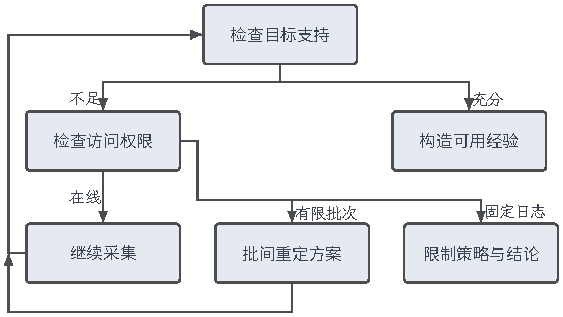
\includegraphics[width=95.282mm]{figures/07-reinforcement-learning/03-task-expansion-and-trustworthiness/tikz/rl-multi-agent-data-loop.pdf}
 \caption{覆盖缺口与记录访问权限决定的处理路径。在线访问允许补采，有限批次只允许批间调整；固定日志不能继续交互，须限制目标或明确引入可检验假设。}
 \label{fig:rl-multi-agent-data-loop}
\end{figure}

有限批次可采用如下协议：总共$B$批，第$b$批包含$N_b$个联合环境步；批内冻结行为策略、伙伴抽样与探索规则，批结束后再按反馈选择第$b+1$批方案。若对手在内部在线适应，须将其适应规则作为策略的一部分声明，并记录所依赖的历史，不能将它称为固定的状态条件对手。只有固定日志时，可将策略限制在有支持的区域、增加可检验结构假设，或按第\ref{chap:rl-information}章采用悲观评价。网络容量再大，也不能从相同日志中区分前述两个奖励模型，因而不能单独解决不可识别性。

% Outline: 7.4
\section{不同参与者依赖下的行为后果估计}
\label{sec:rl-multi-agent-estimation}

联合经验有了明确来源、也确认了覆盖后，估计“某个动作的后果”仍有多种做法，区别在于保留多少参与者之间的依赖。可以把所有人的当前动作都保留下来，估计一个完整的联合价值；也可以固定其他人的动作，只比较我换成别的动作会怎样（个体反事实）；还可以假定联合价值能由各人的局部效用组合而成（局部分解）；或者干脆去预测伙伴会怎么行动，把伙伴的行为显式建进模型；更复杂时，还要计入“我的改变会诱发伙伴如何回应”。这五种估计方式回答不同问题、服务不同计算，可以叠加使用。例如集中训练的评论家可以同时以伙伴类型为条件、又输出固定他人动作后我的全部候选动作价值；群体学习器也可以用单调分解来计算近似的相互响应。

% Outline: 7.4.1
\subsection{基于联合行为的后果估计}
\label{sec:rl-multi-agent-joint-value}

先考虑利用全局状态、联合动作及所需历史的集中评价：固定要评价的联合策略$\bm\pi$，把当前所有人的动作也作为输入，估计一个完整的联合动作价值。做这种集中评价时，评论家用于递推的条件变量$x_t$必须足以预测它会产生的后继过程：完全可观测且策略无记忆时可取$s_t$，策略依赖历史时则要取$(s_t,\bm I_t)$。
\begin{align}
 Q_i^{\bm\pi}(x,\bm a)
 &=\mathbb E[G_{i,t}\mid x_t=x,\bm a_t=\bm a],\\
 V_i^{\bm\pi}(x)
 &=\sum_{\bm a}\bm\pi(\bm a\mid x)Q_i^{\bm\pi}(x,\bm a).
\end{align}
其中$Q_i$评价本次联合动作已确定、随后照$\bm\pi$执行的长期后果，$V_i$还按现有策略平均本次动作。$\bm\pi(\bm a\mid x)$只是在集中条件变量$x$下写出各合法局部策略产生的分布，并未授予行动者读取整个$x$的权限。若现有策略不给某个合法联合动作正概率，其$Q_i$仍可通过从$x$强制执行该动作、随后遵循$\bm\pi$的过程定义；不能用零概率事件上的条件期望唯一确定它。

为从训练样本中的联合转移记录递推这些价值，将回报拆成即时奖励与折扣后的后继回报，再对后继集中条件变量及联合动作取条件平均，得到Bellman评价式
\begin{equation}
 Q_i^{\bm\pi}(x,\bm a)=R_i(x,\bm a)+
 \gamma\sum_{x',d}T_x(x',d\mid x,\bm a)(1-d)
       \sum_{\bm a'}\bm\pi(\bm a'\mid x')Q_i^{\bm\pi}(x',\bm a').
 \label{eq:rl-multi-agent-joint-bellman}
\end{equation}
连续空间中，相应求和改为积分。上式只使用期望的线性分解，没有假设$r_i$、$x'$与$d$条件独立。训练时可用一条完整联合反馈样本替代条件期望，构造
$y_i=r_i+\gamma(1-d)V_{i,\text{目标}}(x')$，再最小化$(Q_{i,\bm\phi}(x,\bm a)-y_i)^2$作TD更新。这里$d$只表示真实终止：终止后没有后继回报，因而乘$1-d$；采样截断但过程未终止时，仍须保留后继价值。日志必须按第\ref{sec:rl-multi-agent-records}节保存或重建与当前接口一致的$x'$。

若要按零和或Nash标准选择后续行为，Minimax-Q将内层策略平均换成零和阶段价值，Nash-Q换成选定均衡的收益。此时进行的是控制备份，而不是对同一个固定$\bm\pi$的评价。即使保留集中训练，也未必需要输入当前联合动作。多智能体深度确定性策略梯度（multi-agent deep deterministic policy gradient, MADDPG）使用动作价值，评价各人的连续动作组合；多智能体PPO（multi-agent PPO, MAPPO）使用状态价值，作为采样回报的比较基准。表\ref{tab:rl-multi-agent-critics}比较这两种评论家接口。

\begin{table}[htbp]
 \centering
 \begin{tabularx}{\linewidth}{@{}l >{\raggedright\arraybackslash}X >{\raggedright\arraybackslash}X@{}}
 \toprule
 方法 & 训练输入与评价对象 & 策略更新与执行\\
 \midrule
 MADDPG & 集中条件变量$x$及$\bm a$；各自$Q_i(x,\bm a)$ & 对自身动作求价值梯度；执行仅用局部输入的确定性行动者\\
 MAPPO & 集中状态或联合观测，可补个体观测或角色标签；$V_i(x)$或团队$V(x)$ & 用回报与$V$构造优势；执行仅用局部输入的随机行动者\\
 \bottomrule
 \end{tabularx}
 \caption{集中动作价值与状态价值的两种接口。联合观测是否足以预测后继过程仍须论证；状态价值评论家不必输入当前联合动作。}
 \label{tab:rl-multi-agent-critics}
\end{table}

MADDPG用集中动作价值指导确定性行动者，可处理合作或竞争收益。MAPPO研究则在合作任务中考察集中状态价值怎样配合PPO，报告的是相应实现条件下的经验表现。两者使用不同评论家，并不意味着集中训练天然优于其他训练权限\scite{rl7-lowe2017,rl7-yu2022}

两种接口都依赖联合轨迹，需承担集中状态与联合历史的传输、价值网络前后向计算和联合轨迹存储成本。这些集中条件变量可帮助区分他人动作的作用，却既不冻结他人策略，也不消除函数逼近误差。尤其当$x$只含当前观测、遗漏对方记忆时，式\eqref{eq:rl-multi-agent-joint-bellman}所需的Markov条件仍可能缺失。训练得到价值之后，行动者还须遵守第\ref{sec:rl-multi-agent-permissions}节的执行权限。

% Outline: 7.4.2
\subsection{基于个体行为反事实的后果估计}
\label{sec:rl-multi-agent-counterfactual}

合作任务里只有一个共同奖励，于是会出现“功劳算谁的”问题：一次成功通过，究竟是因为我主动前进，还是因为对方及时等待？这就是团队中的信用分配。它最干净的形式可以先在一步任务里看清：把入口截成“一次联合动作后立即终止”的独立矩阵任务（故动作价值等于即时奖励），下一小节的表示反例也沿用这一约定。

要量化个人贡献，一种直接的做法是：先规定一个参照动作$c_i$（代表“我本来可以怎么做”），再比较“我实际这么做”和“换成参照、其他人不动”两种情况下的团队奖励之差，称为\term{差分奖励}（difference reward）：
$D_i=R(x,\bm a)-R(x,(c_i,\bm a_{-i}))$。已知上述一步奖励表时，取$c_1=W$得到$D_1=3$。实际交互只执行了一个联合动作，通常没有替代动作的第二份实测结果，而且替代动作还可能改变后继状态。因此，差分的来源须明确为模型、额外试验或价值估计，不能把它作为原日志中已经观察到的事实。

若要指导长期策略更新，需比较候选动作的回报价值，而不只比较即时奖励。反事实多智能体策略梯度（counterfactual multi-agent policy gradients, COMA）用当前策略规定参照：保持其他人的本次动作$\bm a_{-i}$不变，将$i$的候选动作价值按$\pi_i$平均作基线，再与实际动作价值相减：
\begin{align}
 b_i(x,\bm a_{-i})
 &=\sum_{\tilde a_i}\pi_i(\tilde a_i\mid I_i)
       Q^{\bm\pi}(x,(\tilde a_i,\bm a_{-i})),\\
 A_i^{\text{COMA}}(x,\bm a)
 &=Q^{\bm\pi}(x,\bm a)-b_i(x,\bm a_{-i}).
 \label{eq:rl-multi-agent-coma}
\end{align}
例如，1以$1/4$概率前进、$3/4$概率等待且2已等待时，上述一步任务的基线为
$\tfrac14(2)+\tfrac34(-1)=-1/4$，前进的优势为$9/4$。它小于固定以等待为参照的差分3，是因为基线比较当前策略的平均动作，而非固定动作$W$。

依赖别人实际动作的基线，是否会改变策略梯度的期望？先将获准使用的公共信号纳入各$I_i$，并要求给定足以描述联合后继过程的条件变量$x$和其他动作$\bm a_{-i}$后，$i$的条件动作分布仍为$\pi_i(\cdot\mid I_i)$。在策略可微、支持固定且得分与基线的乘积可积时，$b_i(x,\bm a_{-i})$不随本次抽到的$a_i$改变；更新中还须把它视为常数，停止通过基线反向传播。因而可以将它提出动作求和：
\begin{align}
 &\mathbb E_{a_i\mid x,\bm a_{-i}}
   [\nabla_{\bm\theta_i}\log\pi_i(a_i\mid I_i)b_i(x,\bm a_{-i})]\nonumber\\
 &\quad=b_i(x,\bm a_{-i})
       \sum_{a_i}\nabla_{\bm\theta_i}\pi_i(a_i\mid I_i)=0.
 \label{eq:rl-multi-agent-baseline-zero}
\end{align}
最后一步使用概率归一化：$\sum_{a_i}\pi_i(a_i\mid I_i)=1$，对参数求导为零。再平均$(x,\bm a_{-i})$就得到基线项零均值，承接定理\ref{thm:rl-learning-baseline}。若两人共享未记录的随机信号，给定$\bm a_{-i}$后的自身分布可能不再是$\pi_i$，推导中的替换就失效。需要在真实联合策略中处理相关信号，重新推导得分与基线；只将得分改成另一个条件分布的对数梯度，还不足以证明估计的仍是原目标梯度。

为计算该基线，COMA评论家可一次输出自身全部候选动作价值，避免逐个候选运行完整网络。但输出规模仍随$|\mathsf A_i|$增长，连续动作还需近似积分。评论家的训练目标来自联合轨迹，未执行候选的价值仍是估计，而非新增观测。原方法据此将集中评论家与分散行动者连接起来\scite{rl7-foerster2018coma}

零均值结论只保证从精确价值中减去该基线不改变策略梯度期望，并不保证任何基线都降低方差；评论家误差还可能使优势估计失真。此处的“反事实”指固定他人当前动作的候选价值比较，不能据此宣称识别了因果结构模型中唯一真实的个人贡献。

% Outline: 7.4.3
\subsection{基于局部行为组合的后果估计}
\label{sec:rl-multi-agent-factorization}

联合价值回答了“整组动作有多好”，但部署时每个人只能在本地独立选择自己的动作，他既看不到联合价值表、也无法和所有人实时联合优化。于是需要另一种结构：让每个人只计算一个依赖本地历史的局部效用，再保证“每个人都选本地最优”这件事拼起来恰好等于“联合动作最优”。形式地说，设各人只能计算局部效用$q_i(I_i,a_i)$并各自执行$a_i^*\in\arg\max_{a_i}q_i(I_i,a_i)$，所有局部贪心动作能组成联合贪心动作这一性质称为\term{个体与整体最大化一致性}（individual-global-max, IGM）；这里效用是帮助组合团队行为的内部量，不必等于$i$自己的环境回报。

\Needspace{24\baselineskip}
图\ref{fig:rl-multi-agent-mixers}给出两种实现这种一致性的结构。价值分解网络（value decomposition networks, VDN）直接设$Q_{\text{tot}}=\sum_i q_i$，把各人的局部效用相加；单调价值函数分解方法QMIX（monotonic value function factorisation）允许训练状态决定混合器参数，但以非负权重和单调激活保证$\partial Q_{\text{tot}}/\partial q_i\geq0$。提高任一局部效用不会降低联合值，因此部署时可只保留局部贪心选择，无须读取状态。实现这一便利的代价，是分别将联合价值限制为加和或单调组合\scite{rl7-sunehag2018,rl7-rashid2018}

以下充分条件将“不降低联合值”的性质转成对局部贪心动作的保证。

\begin{theorem}[单调组合的局部贪心充分性]
\label{thm:rl-multi-agent-monotone}
固定评论家条件变量$x$及所有局部历史，假设联合动作集合是各人动作集合的笛卡尔积，且局部最大值都存在。若
\[
 Q_{\text{tot}}(x,\bm a)
 =f_x(q_1(I_1,a_1),\ldots,q_m(I_m,a_m))
\]
对每个局部效用逐坐标非减，就有
\[
 \prod_i\arg\max_{a_i}q_i(I_i,a_i)
 \ \subseteq\ \arg\max_{\bm a}Q_{\text{tot}}(x,\bm a).
\]
\end{theorem}
\begin{proof}
任取一组局部最大化动作$\bm a^*$，从任意联合动作$\bm a$开始逐个替换分量。第一分量改为$a_1^*$时，$q_1$不下降，其余效用保持不变；由$f_x$对第一坐标非减，联合值也不下降。第二分量改为$a_2^*$时理由相同，依次完成$m$次替换便有
$Q_{\text{tot}}(x,\bm a)\leq Q_{\text{tot}}(x,\bm a^*)$。由于起点$\bm a$任意，$\bm a^*$最大化联合值；又因为任意局部最大化组合都可作上述替换，故得到所述包含关系。
\end{proof}

保证方向仅从局部最大化指向联合最大化，不能无条件写成等号。例如$f_x$为常数时，全部联合动作都最优，$q_1$却可以只有一个最大化动作；平台区间与并列效用也会造成差别。若合法动作之间存在耦合约束，各人合法动作的乘积可能包含非法组合，逐分量替换就未必保持可行，需重新检验证明条件。

\begin{figure*}[htbp]
 \centering
 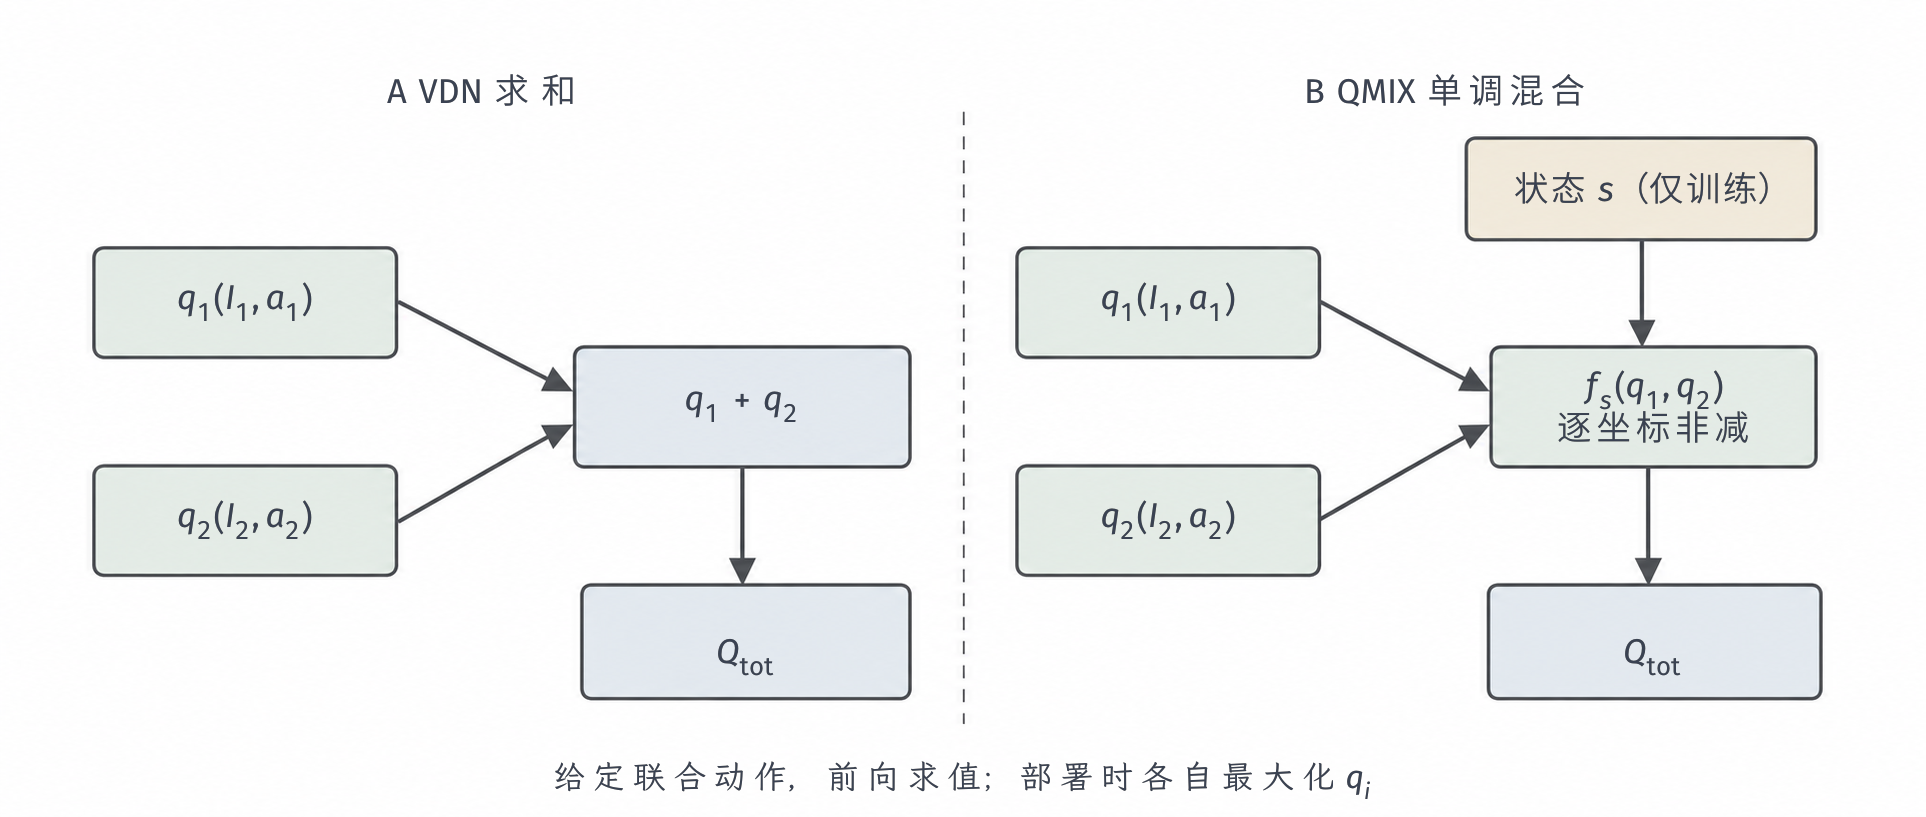
\includegraphics[width=157.400mm]{figures/07-reinforcement-learning/03-task-expansion-and-trustworthiness/generated/rl-multi-agent-mixers/figure.png}
 \caption{给定联合动作时，VDN与QMIX由标量局部效用$q_i(I_i,a_i)$组合联合价值。图中只画前向求值；训练时联合TD损失经求和或单调混合器向全部局部效用网络反传。状态仅供QMIX训练混合器使用，部署时各人选择自身$q_i$的最大化动作。}
 \label{fig:rl-multi-agent-mixers}
\end{figure*}

单调表示的限制也可以在入口一步奖励表中检验。对方前进时，1等待更好；对方等待时，1前进更好，即两列分别要求
$Q(F,F)<Q(W,F)$和$Q(F,W)>Q(W,W)$。若局部排序$q_1(F)>q_1(W)$，第一列违反非减性；若排序相反，第二列违反；若二者相等，单调混合器在两列都不能产生严格差别。因而固定历史下的标量局部效用不能用这一结构精确表示整张表。然而“1前进、2等待”的固定约定仍可分散执行并取得最优奖励。整表可表示、最优动作可执行与训练能找到该动作，是需要分别验证的三件事。

\Needspace{16\baselineskip}
若任务需要更丰富的价值模式，可以放松或改写组合约束，表\ref{tab:rl-multi-agent-factorization}列出两种方式。QTRAN用价值变换和一致性约束保持最优动作；QPLEX以优势分解表示更一般的IGM结构。它们扩大的是表示能力，不是行动者可读取的观测、历史和消息范围。结构在理论上能表示某种值，还须与实际训练是否满足约束、函数逼近误差及优化误差分开判断\scite{rl7-son2019,rl7-wang2021qplex}

\begin{table}[htbp]
 \centering
 \begin{tabularx}{\linewidth}{@{}l >{\raggedright\arraybackslash}X >{\raggedright\arraybackslash}X@{}}
 \toprule
 结构 & 保留的限制或分解 & 代价与边界\\
 \midrule
 VDN & 联合价值为局部效用之和 & 组合便宜；不能表达一般相互作用\\
 QMIX & 状态条件的逐坐标非减混合 & 增加混合器；局部排序不能随他人动作反转\\
 QTRAN & 联合价值与易分解变换在贪心处相等、其他动作满足不等式 & 需拟合联合值并施加约束；近似惩罚不保证精确满足\\
 QPLEX & 局部优势$q_i-\max q_i\leq0$以正权组合，另建联合基准值 & 优势与权重结构增加表达力；表示充分性不等于优化收敛\\
 \bottomrule
 \end{tabularx}
 \caption{局部价值组合的表示限制与代价。更换组合结构不妨碍同时使用伙伴条件化、回放管理或群体训练。}
 \label{tab:rl-multi-agent-factorization}
\end{table}

这些结构都可从联合转移构造团队TD目标，并把损失反传到局部网络。差别在于怎样计算目标中的最大值，以及可以容纳哪些联合价值模式。每人有$A$个动作时，直接枚举需处理$A^m$个组合；局部贪心只比较$mA$个效用，再调用混合器。降低的是动作最大化的计算成本，不能据此断言同样数量的样本足以准确学习所有效用。

% Outline: 7.4.4
\subsection{基于其他参与者策略的行为后果估计}
\label{sec:rl-multi-agent-opponent-model}

前面都假定别人的行为已知，但现实中伙伴的策略通常是隐藏的，只能通过交互去推断。关键的直觉是：即使我当前动作完全相同，不同类型的伙伴也会让后果不同。

要把对伙伴类型的判断写成可更新的概率分布，令伙伴信念$b_t(z)=\mathbb P(z\mid I_{i,t})$，即仅依据获准历史形成的类型分布。自身动作$a_{i,t}$可能改变随后看到的证据$e_{t+1}$，故用$\ell(e_{t+1}\mid I_{i,t},a_{i,t},z)$表示相应似然。若动作只依据已记录历史和独立随机数产生，其选择概率不随候选类型变化，可在贝叶斯归一化时相消。于是用新证据更新信念：
\[
 b_{t+1}(z)=
 \frac{\ell(e_{t+1}\mid I_{i,t},a_{i,t},z)b_t(z)}
      {\sum_{\tilde z}\ell(e_{t+1}\mid I_{i,t},a_{i,t},\tilde z)b_t(\tilde z)}.
\]
此更新要求分母大于0，即至少一个具有正先验概率的类型对所见证据赋予正似然。若动作选择使用了未记录的类型线索，动作概率就不能直接消去。若没有直接观察伙伴动作，似然还须对隐藏动作、状态或消息求和，不能在部署辨识中读取仅供训练的真实动作标签。类型若外生变化，则先通过类型转移核预测，再由证据校正。这里与式\eqref{eq:rl-transfer-belief-update}的贝叶斯步骤相同，变化的是推断对象：从任务条件转为参与者行为。

信念可用于评价候选动作。令$Q_i(I_i,b,a_i,z)$表示固定类型$z$下执行$a_i$，随后按同一套策略及信念更新规则行动的条件回报，则全期望公式给出
$Q_i(I_i,b,a_i)=\sum_z b(z)Q_i(I_i,b,a_i,z)$。
各项都须平均尚未观察的伙伴动作和状态，不能为每个类型偷偷换用“已知类型时”的最优策略，否则平均后不再对应实际可执行行为。后续若继续辨识类型，价值状态与递推也须保留信念更新；把信念冻结的近似会遗漏探测反馈对后续动作选择及回报的影响。

类型模型也可不用有限标签，而用历史编码器输出一个向量，再由该向量预测下一动作的分布。训练时最小化可见动作的负对数似然，即提高模型赋给实际观察动作的概率，学得的表示再输入条件评论家或策略。每次更新需支付历史编码、似然预测及候选动作评价的计算成本，不必直接读取对方网络参数。身份、检查点版本和潜在类型仍不能混为一谈，同一身份可以改用策略，不同身份也可能行为相同。上述估计将对手视为固定或外生变化，尚未计入自身更新诱发的响应。

% Outline: 7.4.5
\subsection{基于参与者相互响应的行为后果估计}
\label{sec:rl-multi-agent-response-model}

比“伙伴类型固定”更进一步的是：伙伴也在学习、会对你的改变作出反应。自身行为改变后，对方可能让步，也可能采用更强硬的规则；只拟合他当前的等待率，就漏掉了“我的策略改变会诱发他如何回应”这一条影响途径。

在两人问题中，固定响应前的对方参数$\bm\psi_0$，以
$\bm\psi'=\mathcal R(\bm\theta_i;\bm\psi_0)$表示对方看到$i$的策略或交互之后采用的参数，$J_{-i}$为对方目标。若$\mathcal R(\bm\theta_i;\bm\psi_0)=\bm\psi_0$，就回到固定对方的估计。若预测对方作一步学习，可规定
$\bm\psi'=\mathcal R(\bm\theta_i;\bm\psi_0)
=\bm\psi_0+\eta\left.\nabla_{\bm\psi}J_{-i}(\bm\theta_i,\bm\psi)\right|_{\bm\psi=\bm\psi_0}$，其中求响应映射对$\bm\theta_i$的导数时保持$\bm\psi_0$固定。这一规则还要求说明它使用的目标、当前策略和用于估计梯度的联合轨迹训练样本。继续增加推理层次时，还须规定对方是否知道$i$的更新规则、是否也预测$i$；增加递归深度会增加假设，而非自动增加准确性。

为区分自身直接改变与对方响应的影响，若$J_i$及$\mathcal R$在所考察邻域可微，可对复合回报使用链式法则：
\begin{equation}
 \nabla_{\bm\theta_i}J_i(\bm\theta_i,\mathcal R(\bm\theta_i;\bm\psi_0))
 =
 \left.\partial_{\bm\theta_i}J_i(\bm\theta_i,\bm\psi)
       \right|_{\bm\psi=\bm\psi'}
 +[D_{\bm\theta_i}\mathcal R(\bm\theta_i;\bm\psi_0)]^\top
 \left.\nabla_{\bm\psi}J_i(\bm\theta_i,\bm\psi)
       \right|_{\bm\psi=\bm\psi'}.
 \label{eq:rl-multi-agent-response-gradient}
\end{equation}
右侧两个回报偏导都在响应后的$(\bm\theta_i,\bm\psi')$处评价：第一项求导时固定$\bm\psi'$，第二项再用响应映射的Jacobian把对方参数变化传回自身参数；$D_{\bm\theta_i}\mathcal R$则在响应前参数$\bm\psi_0$固定时求得。

用一个独立的单步通道变体演示这两条途径。自己以前进概率$p$行动，对方以前进概率$q$行动，给定$p,q$后两人独立随机化；自己前进且对方等待时得1，其余结果得0，一步后终止。因此自身期望回报为$J(p,q)=p(1-q)$。假设对方观察到自己的策略后采用$q(p)=0.8-0.6p$，$p\in[0,1]$；此时$q$始终在$[0.2,0.8]$内。这个响应函数是教学假设，计分也与前面$-1/-4$的通道任务分开。

在内部点$p_0\in(0,1)$，先固定已经响应的$q(p_0)$，直接改变$p$所得导数为$1-q(p_0)=0.2+0.6p_0$。再计入对方前进概率的变化，间接项为$-p_0q'(p_0)=0.6p_0$，两者合计$0.2+1.2p_0$。也可先代入得到$J(p,q(p))=0.2p+0.6p^2$再求导，得到相同结果。若始终把对方固定为$q=0.8$，目标就是$0.2p$，导数才恒为0.2；两种计算对应不同的响应假设。

一步学习响应还需对对方的梯度更新求导，因而涉及梯度的导数；只有交互观测时则要先拟合响应模型，承担相应误差。学习感知的对方学习（learning with opponent-learning awareness, LOLA）据对方学习步骤构造了此类更新\scite{rl7-foerster2018lola}

式\eqref{eq:rl-multi-agent-response-gradient}暂将$\mathcal R$视为确定映射。若它由随机采集的训练样本更新产生，对一份固定样本求导仅得到条件导数；若训练样本的采集律也随$\bm\theta_i$变化，完整期望梯度还包含分布的导数。第\ref{sec:rl-transfer-value-training}节的元学习目标同样区分了固定样本求导与对采样过程求导。

若最佳响应多解或不连续，式\eqref{eq:rl-multi-agent-response-gradient}的可微映射假设可能不成立；对手若不按所设规则学习，求得的导数也只描述错设模型。更深层推理会提高计算成本并放大这种风险。预测下一次响应只是预测任务；斯塔克尔伯格式（Stackelberg）承诺解要求先行者公开承诺策略，后行者据此作最佳响应，因而还须有可承诺、可观察的先后行动协议。同时行动下的Nash均衡又要求固定他人策略后检验单方偏离。三者不能凭响应模型的复杂程度相互替代。

% Outline: 7.5
\section{多智能体的策略更新与学习动态}
\label{sec:rl-multi-agent-learning}

有了价值与优势，还要规定策略如何据此更新，而多智能体的更新比单人多了两个层面的牵连。一个训练批次可以产生价值更新或梯度步；与此同时，各学习者既可以只针对当前对手响应，也可以针对历史上出现过的行为响应；训练对手还可以由一个不断扩充的策略群体来安排配对。例如“从策略库中抽对手，再用策略梯度训练近似最佳响应，最后把新响应加回库”，就同时规定了三件事：更新怎么算（梯度/价值）、相互如何适应（对库中对手）、以及训练群体如何组织（扩充策略库）。下面分别讲清这三个环节，最后再追问：当大家都在同时学习时，这个过程是否稳定、能保证什么。

% Outline: 7.5.1
\subsection{由价值与梯度计算策略更新}
\label{sec:rl-multi-agent-update}

先在本轮计算中冻结其他策略与目标评论家。对训练批次$D_{\mathrm{batch}}$中的联合转移求后继目标，再拟合价值或构造优势，最后得到新动作规则或新策略参数。表\ref{tab:rl-multi-agent-value-updates}按这条路径比较几种价值方法。独立Q学习把他人行为边缘化，只有条件变量足以预测诱导后继过程、诱导环境平稳等前提成立，才能援引表格型单智能体Q学习保证；共同更新、压缩局部历史或使用函数逼近，都可能破坏这些前提。

\begin{table}[htbp]
 \centering
 \begin{tabularx}{\linewidth}{@{}l >{\raggedright\arraybackslash}X >{\raggedright\arraybackslash}X >{\raggedright\arraybackslash}X@{}}
 \toprule
 方法 & 价值输入 & 后继备份 & 动作与执行时可读变量\\
 \midrule
 独立Q & $I_i,a_i$ & 自身$\max Q_i$ & 局部贪心；他人行为被边缘化\\
 Minimax-Q & $s,\bm a$ & 零和矩阵价值 & 按解出的混合策略抽样；需状态\\
 Nash-Q & $s,\bm a$的各人收益 & 选定阶段均衡收益 & 按同一均衡选择约定；需状态\\
 VDN & 局部$I_i,a_i$再求和 & 局部最大值之和 & 每人局部贪心\\
 QMIX & 局部效用与训练状态 & 单调混合的局部最大值 & 每人局部贪心；执行无须状态\\
 \bottomrule
 \end{tabularx}
 \caption{由价值目标生成动作的不同接口。各行仍需规定联合采样、终止处理和目标网络；即使算出了阶段博弈解，也须检查执行所需的状态、观测或公共建议是否可读。}
 \label{tab:rl-multi-agent-value-updates}
\end{table}

一条教学样本即可显示参数化怎样影响更新。设通道样本奖励$r=2$，尚未终止，目标网络给后继联合值1，$\gamma=0.9$，则目标$y=2.9$。当前$Q=1$时，对$\tfrac12(Q-y)^2$作步长0.1的表格梯度下降，残差$-1.9$使新值为$Q'=1.19$。若改用VDN且两个局部效用为0.4和0.6，同一残差分别传到两个表项，一次同步更新后为0.59和0.79，联合值为1.38。联合值的变化不同，是因为两个参数同时改变了有效步长。QMIX传回残差时还须乘混合器对各效用的导数；Minimax-Q与Nash-Q则须为后继目标运行阶段求解器。

随机行动者也可直接沿收益梯度更新。令$\bm\pi_{\bm\theta}=\prod_i\pi_{\bm\theta_i}(a_i\mid I_i)$，暂不共享参数，并固定其他参数与环境机制。假设策略可微、支持固定，同时满足式\eqref{eq:rl-learning-policy-gradient}所需的可积支配条件，以便交换求导与折扣求和。对轨迹概率取对数后，只有$i$的动作项依赖$\bm\theta_i$；每次动作的得分只需乘其后回报，先前奖励对应的得分期望为零。将未来奖励归并为$G_{i,t}$，再用折扣占用表示时刻求和，得到
\begin{align}
 \nabla_{\bm\theta_i}J_i(\bm\pi)
 &=\sum_{t\geq0}\gamma^t
   \mathbb E_{\bm\pi}
   [\nabla_{\bm\theta_i}\log\pi_i(a_{i,t}\mid I_{i,t})G_{i,t}]
 \nonumber\\
 &=\frac{1}{1-\gamma}
   \mathbb E_{x,\bm a\sim d^{\bm\pi}}
   [\nabla_{\bm\theta_i}\log\pi_i(a_i\mid I_i)
           Q_i^{\bm\pi}(x,\bm a)].
 \label{eq:rl-multi-agent-policy-gradient}
\end{align}
这里$d^{\bm\pi}$是集中条件变量$x$与联合动作上的归一化折扣占用度量，它包含归一化因子$1-\gamma$；目标$J_i$未归一化，故第二行须保留$1/(1-\gamma)$。减去符合条件的基线可将$Q_i$换成优势。若联合策略相关，则要从真实联合概率重新推导得分，并检查第\ref{sec:rl-multi-agent-counterfactual}节的基线条件，不能直接使用各人边缘策略的得分。

此梯度把行动者局部历史与评论家集中条件变量的两种用途分开：行动者以自身局部历史计算动作得分，集中评论家提供该动作的长期后果估计。在一步终止的入口教学样本中，若前进概率$p=1/4$由logit参数生成，即以$p/(1-p)$的对数表示参数，采到$(F,W)$并采用前节精确优势$9/4$，得分为$1-p=3/4$，乘积为$27/16$。步长0.1使logit由$\log(1/3)$增至$\log(1/3)+27/160$，前进概率约为0.283。这里直接更新有限一步样本，没有使用归一化折扣占用，因此不额外乘其系数。

\Needspace{7\baselineskip}
PPO类更新用旧策略产生批次，计算自身动作的概率比$\zeta_{i,t}=\pi_i(a_{i,t}\mid I_{i,t})/
\pi_i^{\text{旧}}(a_{i,t}\mid I_{i,t})$，再最大化以下裁剪代理目标的批次均值：
\[
 \min\{\zeta_{i,t}\widehat A_{i,t},
       \operatorname{clip}(\zeta_{i,t},1-\epsilon,1+\epsilon)
                      \widehat A_{i,t}\}.
\]
其中$\widehat A_{i,t}$为优势估计，$0<\epsilon<1$规定围绕概率比1的裁剪宽度；取两项较小值，限制概率比在有利方向上继续扩大代理目标。独立PPO以局部价值估计优势，MAPPO则用集中状态价值。这里的自身概率比没有包含其他动作和后续轨迹，不能等同于完整联合轨迹的重要性比。同批次反复更新所有人时，对手与状态分布均可能变化，所以裁剪机制本身不构成共同学习的单调改进证明。

对连续可微动作，确定性行动者$a_i=f_{\bm\theta_i}(I_i)$可直接对动作价值使用链式法则。精确同策略梯度中的局部方向为
$\nabla_{\bm\theta_i}f_{\bm\theta_i}(I_i)\nabla_{a_i}Q_i^{\bm f}(x,\bm a)$，以归一化$d^{\bm f}$表示时同样带$1/(1-\gamma)$。MADDPG用目标行动者生成后继动作，由联合回放的TD损失拟合$Q_i$，再估计这一方向；用回放分布替代$d^{\bm f}$得到的是离策略代理更新，未经校正不能称为原$J_i$的无偏梯度。COMA保留随机行动者，采用式\eqref{eq:rl-multi-agent-coma}的优势。表\ref{tab:rl-multi-agent-policy-updates}按计算与采样条件比较这些接口。

\begin{table}[htbp]
 \centering
 \begin{tabularx}{\linewidth}{@{}l >{\raggedright\arraybackslash}X >{\raggedright\arraybackslash}X@{}}
 \toprule
 方法 & 价值、采样与策略方向 & 主要成本或失效处\\
 \midrule
 独立PPO & 近期联合轨迹中的局部$V_i$与裁剪得分梯度 & 价值未以其他人的动作或历史为条件；同时更新漂移\\
 MADDPG & 联合回放$Q_i$与确定性动作梯度 & 集中动作输入、回放失配、评论家动作梯度误差\\
 MAPPO & 近期轨迹中的集中$V_i$与裁剪得分梯度 & 集中状态传输、优势误差、批内复用漂移\\
 COMA & 联合$Q$与固定其他动作的候选基线 & 枚举自身候选；未见动作价值估错\\
 \bottomrule
 \end{tabularx}
 \caption{策略梯度接口的价值、采样和成本差异。梯度所针对的$J_i$由收益设定决定，不能由方法名称推断合作或竞争目标。}
 \label{tab:rl-multi-agent-policy-updates}
\end{table}

这些更新只沿图\ref{fig:rl-multi-agent-ctde}的训练梯度路径传递，部署动作仍由各人的局部决策历史及获准消息生成。团队若共享参数$\bm\theta$，每个人的动作概率都依赖它，轨迹得分便为$\sum_i\nabla_{\bm\theta}\log\pi_{\bm\theta}(a_i\mid I_i)$，用于汇总共同$J$的梯度。若各人$J_i$不同而参数仍共享，就须另定加权目标或更新调度。直接平均冲突梯度也已选择了收益取舍，不能视为不改变目标的实现细节。

% Outline: 7.5.2
\subsection{多个学习者之间的相互适应}
\label{sec:rl-multi-agent-mutual-learning}

即使每个学习者各自的更新方向都确定无误，多人一起更新时的“时序安排”仍会显著改变学习轨迹，因为每个人面对的对手都是一个移动目标。这里有一个带点反直觉、但在零和学习中很关键的现象：两个人各自针对“旧的对方”做改进，并不保证他们合起来在向均衡靠近——双方同时迈一步，可能只是在均衡点周围旋转甚至越转越远。下面用最简单的匹配硬币博弈把这种差别算清楚。记$p,q$分别为第一人、第二人选择其第一个动作的概率。
\[
 p^{(k+1)}=[p^{(k)}+\eta(4q^{(k)}-2)]_{[0,1]},\qquad
 q^{(k+1)}=[q^{(k)}-\eta(4p^{(k)}-2)]_{[0,1]}.
\]
若改为交替更新，先计算$p^{(k+1)}$，第二式就使用这一新值而非$p^{(k)}$。图\ref{fig:rl-multi-agent-trajectories}以同一$\eta=0.1$和初值$(0.7,0.5)$迭代两种规则；第三条历史响应曲线则对截至上轮的平均对手求精确最佳响应，平局时选$1/2$。这样可以在同一博弈中区分更新时序和响应对象的影响。

\begin{figure*}[htbp]
 \centering
 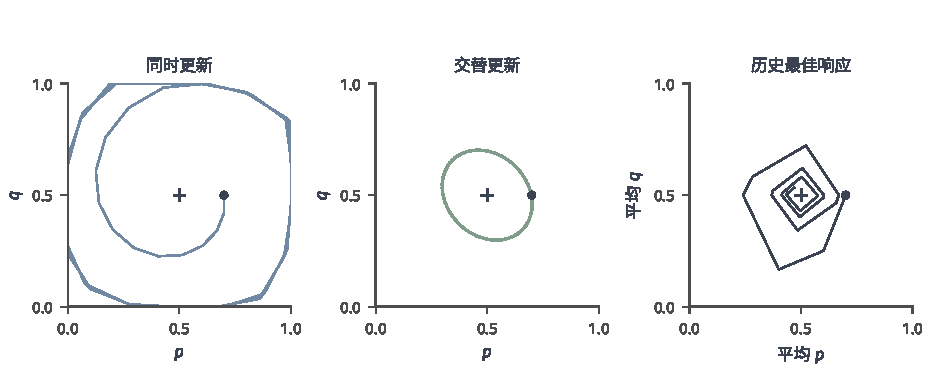
\includegraphics[width=157.400mm]{figures/07-reinforcement-learning/03-task-expansion-and-trustworthiness/matplotlib/rl-multi-agent-trajectories.pdf}
 \caption{匹配硬币博弈中三种响应规则的120次更新。曲线由图源递推式计算，并非实验成绩；圆点标初值，十字标均衡$(1/2,1/2)$，历史响应面板显示累计平均策略。}
 \label{fig:rl-multi-agent-trajectories}
\end{figure*}

在尚未触及投影边界时，令$x=p-1/2,y=q-1/2$表示相对均衡的偏移。同时更新满足
$(x')^2+(y')^2=(1+16\eta^2)(x^2+y^2)$，所以非零偏移在旋转之外还会增大。两人各自针对旧对方改进，并不意味着共同接近均衡。历史响应转而比较整个过去的对手分布，它要减少长期错失的收益，而非只击败最新版本。

要判断这种相互适应长期看是否有效，需要一个比较基准：把自己实际拿到的总收益，与“假如从头到尾固定采用某个动作”能拿到的总收益相比。这个“错失的收益”就是累计外部遗憾，它衡量规则在长期中是否留下了可被持续利用的弱点。
\begin{equation}
 R_i^{(n)}
 =\max_{b_i}\sum_{k=1}^{n}
   [u_i(b_i,\bm a_{-i}^{(k)})
        -u_i(\bm a^{(k)})].
 \label{eq:rl-multi-agent-external-regret}
\end{equation}
最大化在轮次求和之外，意味着$b_i$在所有轮次保持不变。若每轮先取最佳响应再相加，允许替代行为逐轮改变，得到更强的动态比较而非同一遗憾。混合策略版本则用每轮期望收益代替实际动作收益。

用累计遗憾可以直接构造一条很直观的适应规则：过去哪个动作让我错失的收益越多，下一轮就给它越大的选择概率。以$R_i^{(n)}(a)$保存每个固定动作的累计遗憾，记正部为$[r]_+=\max(r,0)$。\term{遗憾匹配}（regret matching）
\[
 \pi_i^{(n+1)}(a)=
 \begin{cases}
 [R_i^{(n)}(a)]_+/\sum_b[R_i^{(n)}(b)]_+,
       &\sum_b[R_i^{(n)}(b)]_+>0,\\
 1/|\mathsf A_i|,&\text{否则}.
 \end{cases}
\]
累计动作遗憾为$(3,-1,1)$时，正部和为4，新分布为$(3/4,0,1/4)$；全非正时，采用均匀回退。上述计算需要所有候选动作的收益，属于已知全部动作收益的更新。已知矩阵可查表，只有实际动作奖励时则需要探索和适当估计，不能将未观测收益直接填入。遗憾驱动的适应规则源于相关均衡学习的工作，第\ref{sec:rl-multi-agent-deviations}节将进一步区分外部与内部偏离保证\scite{rl7-hart2000}

遗憾匹配是在“整个策略”层面比较的；但在序贯博弈（比如前面的隐藏牌游戏）里，完整策略的数量会随决策节点指数增长，逐一比较成本过高。能不能改成在每个信息集局部地评价动作、再把这些局部改进汇总成完整策略的收益？这里有一个关键细节：我自己旧策略很少到达某个节点，不代表“假如我改道去那里”后也很少到达——为了评估改走这条路线的价值，计算局部量时要先把我自己先前的到达概率去掉。

要特别区分这里的“反事实”和前文出现过的两种用法：第\ref{chap:rl-planning}章的规划查询$T(\cdot\mid s,a)$，是在固定规律下预测候选动作的分布；COMA 固定他人当前动作，按自身策略对候选价值取平均作为优势基线；接下来的\term{反事实遗憾最小化}（counterfactual regret minimization, CFR）则保留对方与机会的先前到达概率、只去掉自身先前的到达因子，用局部动作的遗憾来控制完整策略的遗憾。

在图\ref{fig:rl-multi-agent-card-tree}中，将到达历史$h$的概率拆成两部分：$\rho_i^{\bm\pi}(h)$仅乘$i$先前动作的概率，$\rho_{-i}^{\bm\pi}(h)$乘其他人和机会的概率。记终局历史集合为$\mathcal Z$，在$h$强制选$a$、随后按原策略到达$z$的概率为$P^{\bm\pi}(z\mid ha)$，非后继终局取0。先平均后续终局收益，再按对方与机会的到达概率汇总同一信息集中的历史，得到未归一化反事实动作价值：
\begin{align}
 v_i^{\bm\pi}(I,a)
 &=\sum_{h\in I}\rho_{-i}^{\bm\pi}(h)
         \sum_{z\in\mathcal Z}P^{\bm\pi}(z\mid ha)u_i(z),\\
 v_i^{\bm\pi}(I)&=\sum_a\pi_i(a\mid I)v_i^{\bm\pi}(I,a).
 \label{eq:rl-multi-agent-cfr-value}
\end{align}
该式既不乘自身先前到达因子，也不除以$\sum_{h\in I}\rho_{-i}(h)$。它保留的是对方与机会的权重，不是“已到达$I$”之后归一化的普通条件期望。这样的权重将在遗憾分解中与偏离策略的自身到达因子配合，恢复完整策略的收益差。

例如，假定各动作原本均匀，1持$H$、先过牌$K$、2再下注$B$的末级信息集记为$HKB$，其真实到达概率为
$\tfrac12\cdot\tfrac12\cdot\tfrac12=1/8$，反事实权重却为
$\tfrac12\cdot\tfrac12=1/4$，其中删去的是1自身过牌的概率。这样即使1当前很少过牌，仍能比较来到此处后的跟注与弃牌。图\ref{fig:rl-multi-agent-cfr-reach}分开标出这些因子；去掉前序到达因子不同于COMA平均当前自身动作。

\begin{figure}[htbp]
 \centering
 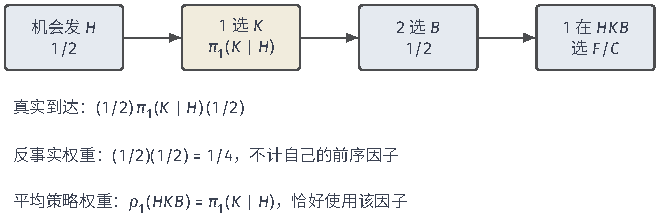
\includegraphics[width=111.651mm]{figures/07-reinforcement-learning/03-task-expansion-and-trustworthiness/tikz/rl-multi-agent-cfr-reach.pdf}
 \caption{高牌信息集$HKB$的真实与反事实到达权重。CFR价值保留机会和2的因子，去掉1的前序选择；用于汇总平均行为策略时，则需要1自身的前序因子。}
 \label{fig:rl-multi-agent-cfr-reach}
\end{figure}

CFR用这些价值在每个信息集运行局部遗憾匹配。一轮完整遍历先冻结$\bm\pi^{(k)}$，从根到叶计算到达因子，再从叶到根汇总式\eqref{eq:rl-multi-agent-cfr-value}。每个动作相对当前局部策略的价值差累加为
\[
 R_i^{(k)}(I,a)=R_i^{(k-1)}(I,a)+
        v_i^{\bm\pi^{(k)}}(I,a)-v_i^{\bm\pi^{(k)}}(I).
\]
遍历结束后，保存当前策略的平均权重，并统一由累计遗憾生成下一轮局部策略，避免同一次遍历混用新旧版本。

表\ref{tab:rl-multi-agent-cfr-round}以零遗憾和全部均匀策略开始，对隐藏牌游戏完成一轮上述计算。原策略期望收益为$J_1=1/8$，表中遗憾与概率均按各行所列动作顺序排列。

\begin{table}[htbp]
 \centering
 \begin{tabular}{@{}llll@{}}
 \toprule
 行动者与信息集 & 动作 & 本轮反事实遗憾 & 下一轮分布\\
 \midrule
 1，持$H$首次行动 & $(B,K)$ & $(3/16,-3/16)$ & $(1,0)$\\
 1，持$L$首次行动 & $(B,K)$ & $(3/16,-3/16)$ & $(1,0)$\\
 1，$HKB$ & $(F,C)$ & $(-3/8,3/8)$ & $(0,1)$\\
 1，$LKB$ & $(F,C)$ & $(1/8,-1/8)$ & $(1,0)$\\
 2，面对$B$ & $(F,C)$ & $(-1/4,1/4)$ & $(0,1)$\\
 2，面对$K$ & $(K,B)$ & $(-1/8,1/8)$ & $(0,1)$\\
 \bottomrule
 \end{tabular}
 \caption{隐藏牌游戏中全树遍历、同步更新的一轮CFR计算。2按自身收益$u_2=-u_1$计算遗憾，故不能直接复用1的收益符号。}
 \label{tab:rl-multi-agent-cfr-round}
\end{table}

以表中$HKB$这一行的计算为例，将终局收益乘上反事实权重，得$v_1(F)=-1/4$、$v_1(C)=1/2$；当前均匀策略值$v_1=1/8$，相减便得$(-3/8,3/8)$。2面对$B$时，高低牌各带对方与机会权重$1/4$，弃牌值为$-1/2$，跟注值为0，均匀当前值为$-1/4$，故只有跟注有正遗憾，下一轮必跟注。其余各行也可由已给的终局收益按同样步骤复算，无须补充游戏规则。

局部遗憾的用途不仅是改变信息集动作。在有限且完全回忆的博弈中，令$\mathcal I_i$为参与者$i$行动的信息集集合，这些局部量还给出完整策略偏离的上界：
\begin{equation}
 R_i^{(n)}
 \leq\sum_{I\in\mathcal I_i}
        \left[\max_a R_i^{(n)}(I,a)\right]_+,
 \label{eq:rl-multi-agent-cfr-bound}
\end{equation}
先用没有对手的两层树看清局部差额怎样相加。根节点选择Stop得到0，选择Go后再选Left或Right，收益分别为2和4。当前策略以$1/2$概率Go，到达下层后又以各$1/2$概率选Left或Right，故旧值为
\[
  \frac12\left(\frac12\,2+\frac12\,4\right)=1.5.
\]
考虑始终Go、随后始终Right的完整偏离，其收益为4。先只改根节点为Go、下层仍按旧策略，收益从1.5提高到3，增益为1.5；再把下层改为Right，收益从3提高到4，增益为1。两个差额相加得到
\[
  (3-1.5)+(4-3)=4-1.5=2.5.
\]
中间的3被消去，留下完整偏离的新旧收益差。下层增益按偏离策略到达下层的概率1计权，而不是按旧策略的到达概率$1/2$计权；否则会漏掉偏离后新增的访问。在博弈中还须保留对方与机会的到达权重，反事实价值正是先保存这部分，再与偏离者自身的到达因子配合。

式\eqref{eq:rl-multi-agent-cfr-bound}的左侧将式\eqref{eq:rl-multi-agent-external-regret}中的固定替代动作扩展为固定完整策略。完全回忆保证同一信息集具有相同的自身前序行动；递归分解收益差时，可以把固定偏离策略的自身到达因子提出信息集历史的求和。该因子介于0和1之间，累计局部增益因而由各信息集最大累计遗憾的正部控制。有限个信息集各自的遗憾增长为$o(n)$时，完整策略遗憾也为$o(n)$。这一结论只支持声明的完整策略偏离类，不能只凭局部观察到的动作收益就假定已取得所有信息集的反事实价值。原始CFR给出了该分解与局部遗憾界\scite{rl7-zinkevich2007}

获得这些局部量仍有成本。全树遍历的每轮计算随访问节点数增长，至少要保存$\sum_I|\mathsf A(I)|$个遗憾项及平均策略累加量。采样CFR可减少单轮访问节点，但需另给采样概率、支持条件，以及无偏反事实估计或相应误差界。任意舍弃罕见分支不能继承全遍历保证，深度近似也会引入拟合误差。

将遗憾界转为均衡保证时，要输出适当的平均策略，而非直接输出最后一轮。在完全回忆下，任取$h\in I$都具有相同的自身前序概率乘积，记为$\rho_i^{(k)}(I)$，不应在信息集内重复累加这一因子。按自身到达概率加权局部动作，得到平均行为策略
\begin{equation}
 \bar\pi_i^{(n)}(a\mid I)=
 \frac{\sum_{k=1}^{n}\rho_i^{(k)}(I)\pi_i^{(k)}(a\mid I)}
      {\sum_{k=1}^{n}\rho_i^{(k)}(I)}.
 \label{eq:rl-multi-agent-average-behavior}
\end{equation}
该比值来自自身序列实现概率的平均：分子对应到达$I$并选$a$的累加概率，分母对应到达$I$的累加概率，二者同时除以轮数后比值不变。逐层应用可恢复均匀抽取整套历史策略时的自身序列概率，而简单逐信息集算术平均通常不能。分母若为零，该信息集在平均实现计划中不可达，可规定任意合法分布，例如均匀分布。

例如，两个版本先过牌概率为0.1和0.9，在$HKB$处跟注概率为1和0。按自身到达加权的平均跟注率为0.1，而非算术平均0.5；它使“过牌再跟注”的自身序列概率为$0.5(0.1)=0.05$，正好等于$\tfrac12(0.1\cdot1+0.9\cdot0)$。若两人零和且各自平均外部遗憾至多$\varepsilon$，这些平均策略的总偏离间隙至多$2\varepsilon$，各人的偏离收益因此也至多$2\varepsilon$。第\ref{sec:rl-multi-agent-deviations}节将用零和消去证明这一结论；它不要求当前策略收敛，也不提供一般和Nash保证。

% Outline: 7.5.3
\Needspace{24\baselineskip}
\subsection{自我对弈与策略群体的迭代组织}
\label{sec:rl-multi-agent-population}

要让“针对历史响应”的学习真正发生，还得有一套训练对手的组织方式，否则很容易在几代之间丢掉重要的检验。比如一个“总让行”策略会被“总前进”克制；可若下一代只针对“总前进”训练、又把“总让行”彻底丢掉，就再也发现不了对手重新变温和时的机会——策略之间常常存在这种循环相克。

把“保留一批历史策略、再针对它们训练新策略”形式化，就得到策略库式的外循环。\term{策略空间响应预言机}（policy-space response oracles, PSRO）用策略库和库上博弈组织这一外循环。
令参与者$i$保存非空有限策略库$\mathcal P_i=\{\pi_i^1,\ldots,\pi_i^{K_i}\}$，其中$K_i\geq1$，每条策略均遵守原任务的观测、消息与行动权限。索引$k_i\in\{1,\ldots,K_i\}$指定一套完整策略。固定初态与交互协议后，库上收益表定义为
\[
 U_i(k_1,\ldots,k_m)
 =J_i(\pi_1^{k_1},\ldots,\pi_m^{k_m}).
\]
它是该组合的期望回报；由有限次对局估计得到的表另记$\widehat U_i$，并保存对局数、伙伴配对及采样随机性。因而估计误差和库中未包含的策略是两种不同限制。元混合策略$\sigma_i$是库索引上的概率分布，决定本回合使用哪套策略；它不同于环境中的$\pi_i(a_i\mid I_i)$，后者决定给定局部历史时采取哪个动作。通常先为一回合抽取一次索引，再执行整套行为策略，不在每一步重新换网络。

图\ref{fig:rl-multi-agent-psro}将库更新展开。先固定元对手$\bm\sigma_{-i}$，响应训练器对该索引分布平均回报，并优化
\[
 \mathbb E_{\bm k_{-i}\sim\bm\sigma_{-i}}
       J_i(\pi_i,\bm\pi_{-i}^{\bm k_{-i}}).
\]
响应器可调用第\ref{sec:rl-multi-agent-update}节的梯度或价值更新；元策略则可由零和求解器、遗憾更新或其他已规定的群体选择规则产生。获得$\hat\pi_i$后，估计其新增收益表项，将它加入库，再重新求元策略。原始PSRO组合的是近似响应训练与经验博弈求解，外循环并不要求响应器采用唯一的底层算法\scite{rl7-lanctot2017}

\Needspace{28\baselineskip}
实际系统未必完整计算上述元博弈，而会按任务选择群体维护方式。与第\ref{sec:rl-multi-agent-collection-plan}节的OpenAI Five版本抽样相比，AlphaStar的联赛训练（league training）设置主学习者和专门寻找其弱点的不同对手角色，再从保留的历史策略中选择训练对手\scite{rl7-vinyals2019}

OpenAI Five则主要维护共同训练的队伍，并混入历史版本对局以减少遗忘，并非为每个队员建立独立的均衡策略库。两种组织分别侧重多角色查找弱点和主训练中的历史检验。增加角色与库策略需要更多对局、存储和维护；这些机制安排了底层强化学习的经验来源，但系统规模本身不能证明已覆盖完整最佳响应。

\begin{figure}[htbp]
 \centering
 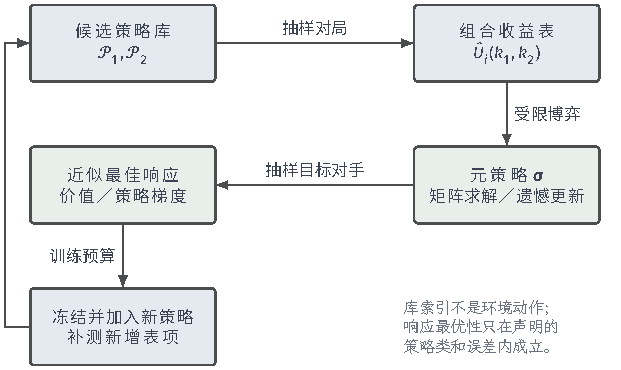
\includegraphics[width=105.184mm]{figures/07-reinforcement-learning/03-task-expansion-and-trustworthiness/tikz/rl-multi-agent-psro.pdf}
 \caption{PSRO的策略库外循环。收益表估计使用对局预算，响应训练使用交互与梯度预算；元策略规定响应对象，响应器规定底层更新计算。}
 \label{fig:rl-multi-agent-psro}
\end{figure}

策略库的限制可由三套抽象教学策略$\alpha,\beta,\chi$说明。以第一人的策略为行、第二人的策略为列，两人的索引都按$\alpha,\beta,\chi$排列，第一人的零和收益表为
\[
 \bm U=
 \begin{pmatrix}0&-1&1\\1&0&-1\\-1&1&0\end{pmatrix}.
\]
从表中可见，$\beta$必胜$\alpha$，$\chi$又必胜$\beta$，没有一套最强纯策略。若双方库只有$\{\alpha,\beta\}$，元解都选$\beta$，库内没有获利偏离；库外的$\chi$却能取得1。加入全部三套策略后，均匀混合使各行收益都为0。这区分了击败当前对手、求解已有收益表中的均衡和覆盖所有可能响应：前两项成立，第三项仍可能失败。

若双方库各有$K$套策略，每格评价$E$局，完整收益表就需$K^2E$场；增加一行一列还须补测相关组合，多方全组合表的项数则为$\prod_iK_i$。响应网络、检查点及响应训练与收益估计的对局记录也占用预算。收益估计误差、响应搜索误差及库外策略都会使元博弈与完整博弈不同，因而受限元解不能单独认证完整博弈不可利用。

% Outline: 7.5.4
\subsection{学习动态的稳定性与保证对象}
\label{sec:rl-multi-agent-stability}

更新怎么算、对谁响应、训练群体如何组织，三者合起来决定了学习动态，因此任何“会收敛/很稳定”的声明都必须对应这一完整组合，换掉其中一个模块结论就可能失效——例如把精确的表格遗憾更新换成误差不受控的神经网络近似，原来的收敛定理就不再适用。表\ref{tab:rl-multi-agent-dynamics}列出各组合实际能保证的输出对象。

\begin{table*}[htbp]
 \centering
 \begin{tabularx}{\linewidth}{@{}l l l >{\raggedright\arraybackslash}X >{\raggedright\arraybackslash}X >{\raggedright\arraybackslash}X@{}}
 \toprule
 更新接口 & 响应规则 & 训练群体 & 当前策略表现 & 平均策略表现 & 保证条件\\
 \midrule
 梯度 & 同时追随 & 当前双方 & 可旋转或发散 & 局部改进不足以保证平均间隙下降 & 另需步长、博弈与算子条件\\
 精确响应 & 历史平均 & 历史策略 & 可持续变化 & 有限两人零和的经典虚构博弈平均可收敛 & 精确响应、完整有限博弈；近似误差另计\\
 局部遗憾 & 同步CFR & 当前与平均 & 不要求收敛 & 适当平均的零和间隙受遗憾界控制 & 有限、完全回忆、正确价值或采样误差控制\\
 梯度响应器 & 元策略响应 & PSRO策略库 & 新响应未必稳健 & 元混合只解受限经验博弈 & 收益表误差、响应误差及策略类限制均需报告\\
 \bottomrule
 \end{tabularx}
 \caption{更新计算、响应规则和群体组织共同确定的保证。当前策略、平均行为策略与库上的元混合策略对应不同输出，应分别报告。}
 \label{tab:rl-multi-agent-dynamics}
\end{table*}

为直观区分这些输出，图\ref{fig:rl-multi-agent-stability}沿用匹配硬币和同一初值，计算交替更新轨迹。固定当前$(p,q)$，两人分别求最佳响应得到总单方偏离间隙
$g(p,q)=|2p-1|+|2q-1|$；检验平均策略时，则代入历轮$p,q$的均值。图中另按固定动作在整段历史上的错失收益计算
\[
 \frac1n\max\!\left\{0,\
 \left|\sum_k(2q^{(k)}-1)\right|-\sum_k u^{(k)},\
 \left|\sum_k(2p^{(k)}-1)\right|+\sum_k u^{(k)}\right\},
\]
这是两人累计平均外部遗憾正部中的较大值，其中绝对值来自比较两个固定纯动作。三条曲线使用同一序列，当前间隙波动时，平均间隙仍可下降。有限步长下遗憾还可能保留偏差，因此图形只能展示所给递推的有限轮次结果，不能据形状断言任意精度收敛。

\begin{figure}[htbp]
 \centering
 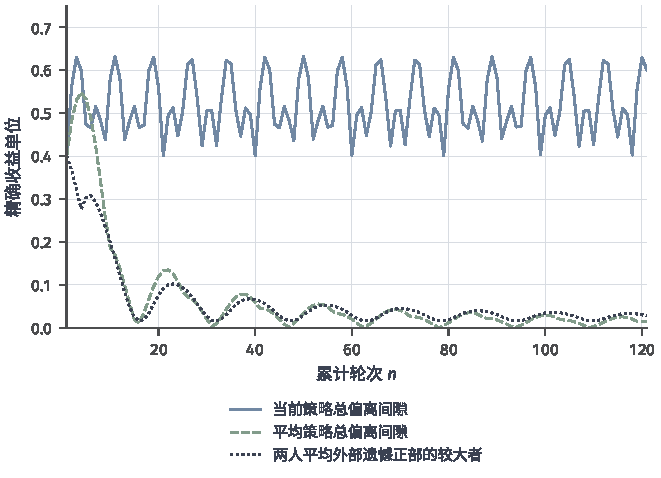
\includegraphics[width=112.000mm]{figures/07-reinforcement-learning/03-task-expansion-and-trustworthiness/matplotlib/rl-multi-agent-stability.pdf}
 \caption{同一交替梯度序列的三种检验量。当前间隙、平均策略间隙与累计平均遗憾均由精确矩阵收益计算，图源保留递推及统计公式，不代表学习基准的实验成绩。}
 \label{fig:rl-multi-agent-stability}
\end{figure}

判断保证能否沿用，需要定位每项误差作用的位置：评论家和采样误差改变收益或梯度估计，近似响应误差改变每轮与最佳响应的比较，共同学习改变下一批交互记录的分布，不完全回忆破坏信息集分解，库外策略则不在元博弈的比较类中。低外部遗憾要进一步控制平均边际策略的Nash间隙，须利用两人零和的收益抵消。一般和中通常只能得到保留相关性的联合经验分布结论，不能按相同证明推出平均独立策略达到Nash均衡。

即便阶段博弈做到了无悔，改变早先动作还会改变后面访问哪些状态。只在已访问位置比较动作，不能控制新策略将到达的位置及其后续回报。需要把后继价值向前传播，同时为未充分探索的位置保留余量。\term{V学习}（V-learning）把状态价值估计、探索与各人的局部对抗老虎机连接起来，并用训练历史构造完整的策略输出。

考虑正整数$H$和有限状态、行动空间，所有参与者在阶段$t=0,\ldots,H-1$行动前共同看到当前状态。每回合都从同一初态生成规则重新开始，转移与奖励规律可以随阶段$t$变化，但在训练回合间固定；每步奖励满足$r_{i,t}\in[0,1]$，第$H$步后终止。这里评价不折扣的整回合回报$\mathbb E\sum_{t=0}^{H-1}r_{i,t}$，与前面的无限折扣目标分开。因此，阶段$t$之后最多还有$H-t$单位回报；这一已知上界正是初始化与截断的依据。

每个参与者$i$为每个$(s,t)$保存状态价值$V_{i,t}(s)$、访问计数和一个只选择自身动作的\term{对抗老虎机}（adversarial bandit）子程序。第~\ref{sec:rl-learning-contextual}~节已说明，它用所选动作的反馈调整动作分布，以应对随历史变化的损失；此处损失会随其他人的学习而变化，不要求环境中另有恶意攻击者。价值初值为$H-t$，终端价值$V_{i,H}=0$。在$(s,t)$第$n\geq1$次访问、取得$r_i$和$s'$后，更新为
\begin{equation}
 \begin{aligned}
  \alpha_n&=\frac{H+1}{H+n},\\
  \widetilde V_{i,t}(s)&\leftarrow
      (1-\alpha_n)\widetilde V_{i,t}(s)
      +\alpha_n\bigl[r_i+V_{i,t+1}(s')+b_{i,n}\bigr],\\
  V_{i,t}(s)&\leftarrow\min\{H-t,\widetilde V_{i,t}(s)\}.
 \end{aligned}
 \label{eq:rl-multi-agent-v-learning}
\end{equation}
$\widetilde V$同样从$H-t$初始化，$b_{i,n}\geq0$是按遗憾与采样误差选取的探索余量；它使未充分采样的后果保持乐观，截断则保留已知回报上限。访问次数$n$决定更新权重，并非环境时刻$t$。局部动作子程序收到已选动作及损失$(H-r_i-V_{i,t+1}(s'))/H$，再更新自身动作分布。由于$0\leq r_i+V_{i,t+1}(s')\leq H-t\leq H$，该损失在$[0,1]$内；未选动作的损失并未全部观测，须由带相应加权遗憾保证的bandit更新处理。价值表因而不必按联合动作展开，但每个人仍需保存自己的动作概率与历史策略。

式~\eqref{eq:rl-multi-agent-v-learning}~的更新权重也规定了策略怎样混合。对已有$n$次访问的位置，第$j$次访问的历史权重为
\[
 \omega_{n,j}=\alpha_j\prod_{\ell=j+1}^{n}(1-\alpha_\ell),
 \qquad j=1,\ldots,n,\qquad\sum_{j=1}^n\omega_{n,j}=1.
\]
例如$H=2,n=2$时，$\alpha_1=1,\alpha_2=3/4$，历史权重为$(1/4,3/4)$；两份局部策略选择某动作的概率若为0.2和0.8，该次混合概率就是0.65，既不是最后一份策略的0.8，也不是均匀平均的0.5。这只演示一次局部混合。完整输出先均匀抽取训练回合索引，在每个到达的状态—时刻对，再按该索引之前的访问记录和上述权重抽取历史回合，按该回合的策略快照选择当前动作，并把抽到的索引带入下一步继续回退；未访问位置需保留初始化策略。必须保存相应计数与策略快照，不能将这一递归协议换成均匀抽取某一回合策略后整局不变。该输出一般依赖历史，不是只读取当前状态的最后一轮策略。

均衡目标决定局部遗憾和联合输出的要求。两人零和时，各人独立执行这一历史输出协议，所得乘积策略可有近似Nash保证。多人一般和时，加权外部遗憾控制对应近似CCE；若改用控制动作替换映射的加权交换遗憾子程序，则可取得近似CE。一般和的联合输出还须在执行前共享一次随机种子，同步各步抽取的历史索引，以保留所需相关性，各人的动作仍由各自策略产生。训练分散执行，并不意味着执行时可以删掉这个公共随机协议。

零和任务可按已知奖励界作正尺度变换与常数平移，采用$r_{2,t}=1-r_{1,t}$的单位区间常和计分。固定$H$时，这种等价编码保留最佳响应与均衡策略，收益误差则须按新旧尺度换算。

在上述有限表格、共同可见状态与单位区间奖励条件下，采用原论文给出的加权正则化跟随领头者（follow-the-regularized-leader, FTRL）子程序，按累计损失估计与正则项选择下一动作分布，并配合相应探索余量及完整历史输出协议。令$n_S=|S|$、$n_{A,\max}=\max_i|\mathsf A_i|$。对$\varepsilon>0$和$\delta\in(0,1)$，两人零和的$\varepsilon$-Nash与一般和的$\varepsilon$-CCE都可在
$\widetilde O(H^5n_Sn_{A,\max}/\varepsilon^2)$个训练回合后以至少$1-\delta$的概率取得；加权交换遗憾版本取得$\varepsilon$-CE的对应量级为
$\widetilde O(H^5n_Sn_{A,\max}^2/\varepsilon^2)$。这里$\varepsilon$按归一化逐步奖励的整回合收益衡量，$\widetilde O$隐藏包括失败概率和参与者数在内的对数因子，一回合至多$H$个环境步。动作规模由联合空间的乘积变为最大单人动作数，是这类结论的关键；它没有保证最后一次策略收敛，也不能直接推广到局部观测、任意神经近似或随意选取的探索余量。具体子程序与输出条件见原论文算法1、3及定理5--7\scite{rl7-jin2021vlearning}

从训练对手表现到元博弈，再到完整策略空间的最佳响应，所需验证范围逐步扩大，训练却未必自然完成这些检验。恶意通信、对抗攻击和安全约束还会改变行为要求，第\ref{chap:rl-trustworthy}章另作讨论。即便当前训练曲线稳定，也不能据此获得这些新目标的保证。

% Outline: 7.6
\section{多智能体的参与者变化适配}
\label{sec:rl-multi-agent-adaptation}

前面所有讨论都默认参与者的人数、伙伴和接口是固定的。部署时这些前提经常变化：机器人团队可能临时增加人手，合作伙伴可能换成一套从未配合过的陌生策略，竞争者也可能采用全新的行为机制。这些是性质不同的适配问题，可以沿用第\ref{chap:rl-transfer}章的训练分布、留出条件和适应预算框架，但必须把“参与者如何变化”明确写进去。跨规模、跨伙伴、跨对手分别改变的条件不同，不能因为在一种变化下协调成功，就同时声称具备了另外两种适配能力。

% Outline: 7.6.1
\subsection{参与者规模变化下的跨规模适配}
\label{sec:rl-multi-agent-scale}

先看人数变化。参与者增加时，原来为固定人数设计的策略可能连输入格式和协作约定都无法复用。例如两人网络若用固定槽位拼接“对方的位置”，就没有放入第三人的槽位；“1 先走、2 后走”的约定也没有规定第三人何时行动。

连续控制还须说明“一个参与者”控制什么。分解式多智能体集中策略梯度（factored multi-agent centralised policy gradients, FACMAC）所用多智能体MuJoCo任务按关节组控制同一系统；更换分组或观测半径会改变各人的动作集合和可见观测范围。此时即使人数相同，任务接口也可能不同，不能只比较参与者数量\scite{rl7-peng2021facmac}

对角色与动作编码相容的参与者，若编号只用于登记身份，重编号就不应改变各物理参与者的决策。把$m$人的动作前可见特征排成$\bm X\in\mathbb R^{m\times d}$，每行对应一人；邻接矩阵$\bm B\in\mathbb R^{m\times m}$记录可用的交互边。固定参数的图策略$F(\bm X,\bm B)$逐行给出各人的动作分布参数，各行使用同一动作编码。令$\bm M$为$m\times m$置换矩阵，同时重排特征行与邻接矩阵的行、列。若
\[
 F(\bm M\bm X,\bm M\bm B\bm M^\top)=\bm M F(\bm X,\bm B),
\]
就具有\term{置换等变性}（permutation equivariance）：先重编号再求策略，等于先求策略再相应重排结果。例如交换1、2两人的编号后，原1对应的策略分布应出现在新2的位置，而不是强迫两人使用相同动作。角色特征也必须随物理参与者一起重排。这是消除任意编号影响的结构要求；能够处理变长有序列表的策略不必满足它，因此变长计算与重编号对称是不同性质。

共享的邻域消息函数与不依赖邻居排列的聚合器，可以构造这种图策略：
\[
 \bm z_i=\operatorname{Agg}_{j\in\mathcal N_i}
           \phi(I_i,I_j,e_i,e_j),\qquad
 \pi_i(\cdot)=f_{\bm\theta}(I_i,e_i,\bm z_i),
\]
其中$\mathcal N_i$为$i$的邻居集合，$\phi$将一对参与者的局部特征映为消息向量，$\bm z_i$为聚合结果；此处$e_i$表示可见角色，不是任意编号，$\operatorname{Agg}$可取不依赖邻居排列的求和、均值或邻居集合上归一化的注意力。空邻域须规定合法输出，例如零向量，才能在所有图上计算策略；按身份槽位拼接一般不具有上述性质。图\ref{fig:rl-multi-agent-graph}展示同一物理图重编号后的对应。部署聚合只能使用本轮动作前实际收到的邻居消息及协议允许共享的字段，不能因图结构可写而假定邻居历史全部可见。

\begin{figure*}[htbp]
 \centering
 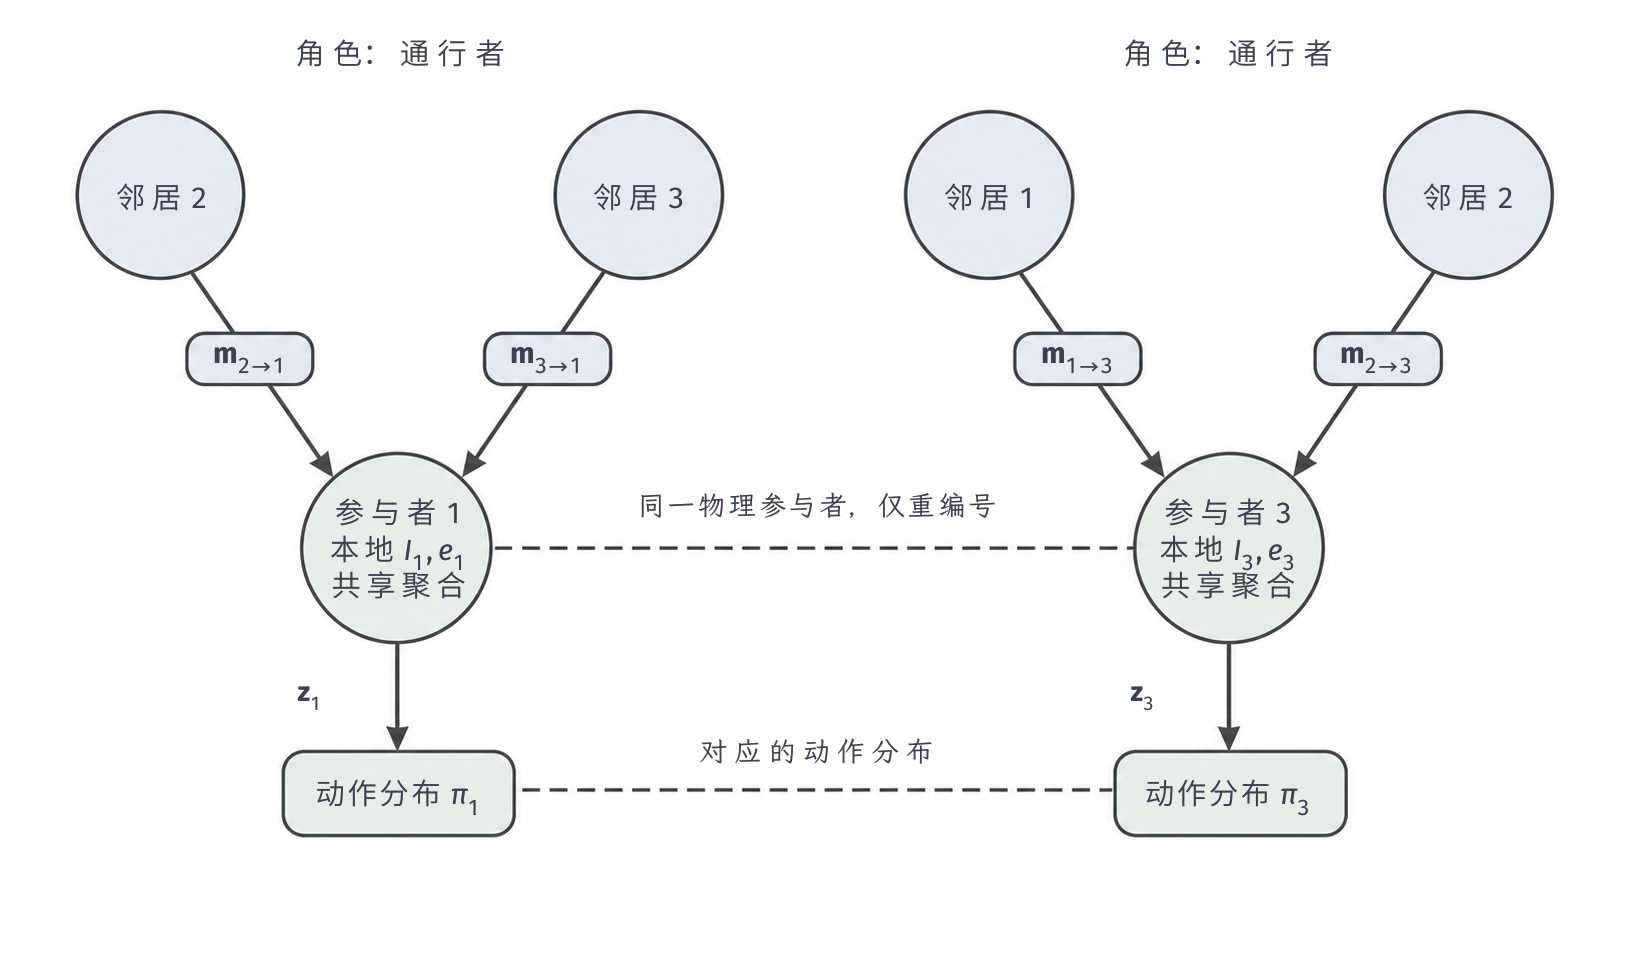
\includegraphics[width=157.400mm]{figures/07-reinforcement-learning/03-task-expansion-and-trustworthiness/generated/rl-multi-agent-graph/figure.png}
 \caption{共享邻域聚合对重编号的响应。实线把邻居消息送至本地主体，再形成动作分布；左右图仅重排同一物理节点的编号。横向虚线连接重编号前后的同一主体及相应动作分布，不是额外通信边；通行任务不变。}
 \label{fig:rl-multi-agent-graph}
\end{figure*}

当邻居很多时，逐个建模“我和每个邻居的交互”成本太高，一个自然的近似是只看群体或邻域的平均行为，把所有他人的联合影响压缩成一个“平均动作”。平均场多智能体强化学习（mean field multi-agent reinforcement learning）
\[
 \bar{\bm a}_{-i,t}
 =|\mathcal N_i|^{-1}\sum_{j\in\mathcal N_i}\bm e(a_{j,t}),
\]
其中$\bm e(a_{j,t})$为动作独热向量，求平均后得到时刻$t$实际执行后的邻域动作频率。空邻域另约定$\bar{\bm a}_{-i,t}=\bm0$，这只是无邻居标记，不是概率分布。同时行动时，参与者提交$a_{i,t}$之前不能读取尚未产生的$\bar{\bm a}_{-i,t}$；执行策略必须改用事前可得的估计$\widehat{\bar{\bm a}}_{-i,t}$。协议可以规定它由上一时刻已观察的均值、邻居策略预测，或同步求解的自洽平均场得到，但训练和评价须固定同一种构造；若通信直接公开本轮意图动作，则应把这项额外权限写入历史。已完成的联合转移可用实际$\bar{\bm a}_{-i,t}$训练评论家，而下一步TD目标中的聚合量须按同一事前规则构造$\widehat{\bar{\bm a}}_{-i,t+1}$。学习器据此将聚合行为作为$Q_i(I_i,a_i,\bar{\bm a}_{-i})$的条件。若后继目标只把事前点估计代入非线性评论家，这里采用的是点代入近似；若要计算对未来实际均值的条件期望，还需对其预测分布采样或积分。训练与评价应保留同一近似口径。原始平均场方法沿这一路线给出Q学习和行动者—评论家机制\scite{rl7-yang2018meanfield}

共享图策略可继续由联合轨迹和团队目标训练，并在训练中覆盖不同图与规模，执行时按当前邻域组装输入。令$E_G$为图边集，每轮沿各边计算消息需要$O(|E_G|)$次函数调用，传递$L$轮则乘$L$；这是固定单条消息计算结构时的调用数，不是整个网络的运行时间。网络能接受变长输入，只解决计算可定义的问题，不保证新人数$m$下回报不降。聚合方式也决定哪些局部特征差别仍可区分：求和随人数变化，均值可能丢掉邻居数量，即便置换等变也可能需要显式计数或密度特征。

平均场近似还要求个体影响较弱、聚合量足以描述交互，仅人数多并不充分。窄通道中一个关键参与者就能完全堵塞，平均前进率却未必指出谁占据瓶颈。异质角色、强配合或拓扑突变也可能使聚合量不足，所以近似有效性仍须在留出规模与交互条件下检验。

% Outline: 7.6.2
\subsection{未见合作者条件下的零样本协调与在线适配}
\label{sec:rl-multi-agent-new-partners}

换伙伴和换人数是两回事：人数不变、只换一个合作伙伴时，最容易出问题的不是技能，而是双方默认的协调约定是否兼容。

Overcooked的共享烹饪任务中也有这种区别。同一厨房下，与共同训练的伙伴完成分工，不代表能与新伙伴保持同样配合；评价须给出伙伴来源，并规定双方是否允许适应\scite{rl7-carroll2019}

先按第\ref{sec:rl-transfer-budget}节区分零样本与适应预算。本章对\term{零样本协调}（zero-shot coordination）采用同样的严格预算口径：不使用新伙伴反馈作伙伴特定的参数更新、记忆适应、类型辨识或模型选择，但可读取已给角色、约定及正常控制所需的观测。在给定任务和伙伴模型下估计当前位置，仍属普通状态估计；利用伙伴动作或回报改变对其行为类型的判断，则已发生适应。即使这一判断只在首回合内更新、网络参数始终固定，也不能按本章口径称为零样本。

文献中的zero-shot coordination有时主要强调测试伙伴未与当前策略共同训练；是否允许首回合内利用伙伴反馈，还须读取具体协议。将这些结果按本章分类时，应按实际反馈、记忆重置与参数更新权限归类。

\term{临时团队协作}（ad hoc teamwork）研究未预先共同训练或充分协调的新队伍，协议可以允许交互辨识和伙伴适配。为确定其可行策略，实验须说明是否共享左右约定、能否通信、角色是否可见、允许试探几步，以及试探失败的代价。任务名称并不自动提供这些权限。

机制选择须与可读任务约定、伙伴类型线索和交互历史对应。扩大训练伙伴群体要有多类伙伴可供交互，处理对称性要知道哪些变换保持任务不变，伙伴条件策略要有部署时可见的类型线索，在线信念更新则要有能区分类型的历史。Other-Play利用所给任务对称性，减少策略对某次自我对弈任意约定的依赖；作用范围仍由该对称性与协调条件限定，不能保证兼容任意未知伙伴\scite{rl7-hu2020otherplay}

一种在线协议先冻结基础策略与类型模型，在前$B$步用获准动作或消息收集证据，再按第\ref{sec:rl-multi-agent-opponent-model}节更新信念，以伙伴条件价值选动作。若还允许梯度适配，须另计更新次数和目标伙伴交互训练记录的来源。报告应区分零样本、仅记忆或信念适应、参数适应，并说明回合内及跨回合的记忆保留。适应后评价可继续估计物理状态，但只要反馈仍修正伙伴类型，适应过程就没有结束；若两者无法分离，也应据实计入协议。交互数量增加不保证类型可辨识，证据不足时仍可能无法区分伙伴。

最后，分工还受观测、历史和角色信号的对称性限制。双方若使用同一确定性策略、取得同一历史，又没有身份、方位或指定不同角色的公共信号，所选动作就相同，无法保证恰好一人前进。独立随机化提供打破对称的机会，却不能保证本轮形成指定分工。合法公共角色信号能改变可行策略集合，因此使用它时须在评价协议中明示。

% Outline: 7.6.3
\subsection{未见竞争者条件下的策略适应}
\label{sec:rl-multi-agent-new-opponents}

面对新竞争者，还要在“针对已知弱点尽量榨取收益”和“对手一变也不至于被反制”之间权衡。

对手条件策略可以先在训练群体中学习行为表示，部署时据可见动作、回合结果或消息更新类型信念，再选择响应。优化目标可以是给定对手分布下的收益，也可以另加已知策略类中的最坏情形限制；比较适应速度前必须先说清使用哪种目标。表\ref{tab:rl-multi-agent-opponent-adaptation}列出相应比较对象，并区分固定对手与随自身行为响应的对手。

\begin{table}[htbp]
 \centering
 \begin{tabularx}{\linewidth}{@{}l >{\raggedright\arraybackslash}X >{\raggedright\arraybackslash}X@{}}
 \toprule
 问题 & 对手、历史及允许更新 & 比较对象\\
 \midrule
 固定对手最佳响应 & 目标固定；可交互观测；按给定预算更新 & 同一对手下可行最佳响应收益\\
 群体内适应 & 见过类型的新抽样；允许历史辨识或少量更新 & 同预算的群体条件基线及零样本策略\\
 跨对手泛化 & 未见行为类型；历史与反馈权限明确 & 留出类型的平均、尾部及最坏已测收益\\
 反应型对手适应 & 对方可随自身行为改变；响应历史需记录 & 声明响应协议下的序贯收益，非固定对手值\\
 \bottomrule
 \end{tabularx}
 \caption{对手适应的目标与可用证据。需同时给出类型留出、记录采集与访问权限和比较对象；同一策略只更换随机种子并未构成类型留出。}
 \label{tab:rl-multi-agent-opponent-adaptation}
\end{table}

例如，规定20场探测再评价100场时，还须确定探测是否计分、记忆是否重置、梯度步上限，以及对手在全部120场中是否保持不变；这些数字仅定义教学预算。响应训练使用的对局不能同时充当独立测试。对手若先以温和行为诱导信念、随后切换，或在探测中继续学习，固定类型模型就可能不适用。此时须按第\ref{sec:rl-multi-agent-response-model}节重新规定响应机制，不能保留固定类型识别的保证。

% Outline: 7.6.4
\subsection{参与者变化适配的泛化与扩展边界}
\label{sec:rl-multi-agent-generalization}

无论测试跨规模、跨伙伴还是跨对手的适配，都应先声明究竟变化了哪个因素，并据此划分训练、验证与测试的参与者及交互记录；把多种变化混在同一批“新环境”测试里，成功或失败都无法归因。

\begin{table}[htbp]
 \centering
 \begin{tabularx}{\linewidth}{@{}l >{\raggedright\arraybackslash}X >{\raggedright\arraybackslash}X@{}}
 \toprule
 变化因素 & 可声明的留出方式 & 必须控制或记录\\
 \midrule
 数量与密度 & 训练2至4人，测试6人等独立设定 & 通道容量、拥挤度、邻域大小，不能只改$m$\\
 身份与组合 & 已见类型的新排列、新搭配 & 角色是否同构；是否共享编号约定\\
 合作者或对手类型 & 留出训练流程、策略家族或行为机制 & 零样本／适应预算；伙伴是否继续学习\\
 收益关系 & 固定关系内的新参数，或另测关系改变 & 团队转竞争已改变目标，不能仅称身份泛化\\
 通信与拓扑 & 留出图、延迟、带宽或接收范围 & 部署消息是否可得；公共信号是否保留\\
 \bottomrule
 \end{tabularx}
 \caption{参与者变化的留出方式与控制条件。支持内的新搭配和未见行为类型不是同一种测试，其覆盖与辨识要求不同。}
 \label{tab:rl-multi-agent-splits}
\end{table}

同一批伙伴更换环境种子，只检验给定伙伴下的运行随机性；同一策略更换编号，至多检验身份依赖。若同时改变人数、角色、奖励和通信，失败不能单独归因于规模，成功也难以辨认是哪项适配有效。因此应先作单因素留出，再评价明确的组合变化，结论范围始终受实际留出因素限定。

% Outline: 7.7
\section{多智能体的行为评价和验证}
\label{sec:rl-multi-agent-evaluation}

最后是评价。多智能体系统的“好”有多个互不替代的侧面，必须分别检验：策略取得了多高的收益？是否满足选定的行为标准（有没有单方面偏离的动机）？能否和声明范围内的新伙伴、新对手正常交互？又花费了多少资源？基准回报说明任务表现，偏离搜索检查稳定性，交叉配对检查约定是否兼容，资源统计说明代价。把这些量压成一个无条件的单一排名，会丢掉各自的验证范围。

% Outline: 7.7.1
\subsection{共同评价目标下的效用、福利与公平评价}
\label{sec:rl-multi-agent-welfare}

评价收益时应先回到各方原本的目标，不能用一个总分掩盖分配差异。

例如，教学结果$(10,0)$与$(5,5)$总收益都为10，最小收益分别为0和5，个体收益的总体方差分别为25和0。若第一种结果总由同一人承担成本，只报团队总分便看不到差异；若角色按公平规则轮换，还需区分单回合和长期分配。实际评价应至少报告均值、分布与失败率，并定义失败究竟是碰撞、超时还是某人的任务未完成。

指标还须对应具体任务接口，表\ref{tab:rl-multi-agent-benchmarks}为此区分环境库中的任务。例如，星际争霸多智能体挑战（StarCraft multi-agent challenge, SMAC）考察局部观测下的团队微操，即多个受控单位分别选择移动、攻击等战斗动作；地图和敌人脚本共同决定难度与胜率含义，不能只写环境库名称来确定评价条件\scite{rl7-samvelyan2019}。表中的MPE指多智能体粒子环境（multi-agent particle environment），其收益、观测与通信同样由具体任务配置决定。

\begin{table*}[t]
 \centering
 \begin{tabularx}{\linewidth}{@{}l >{\raggedright\arraybackslash}X >{\raggedright\arraybackslash}X >{\raggedright\arraybackslash}X >{\raggedright\arraybackslash}X@{}}
 \toprule
 具体接口 & 合作或竞争结构 & 可用观测 & 通信条件 & 主要指标\\
 \midrule
 SMAC，3m & 三个受控单位合作，对抗脚本敌人 & 各自视野内的单位特征；训练可给全局状态 & 原任务无额外学习消息，新增须声明 & 地图胜率、回报、超时率\\
 MPE，simple\_spread & 多个体覆盖地标；局部碰撞项与共享项比例需指定 & 自身及其他实体的配置相关特征 & 此任务的静默体无消息；不能外推至其他MPE任务 & 覆盖距离、碰撞及所定奖励\\
 Overcooked，cramped\_room & 两人完成共享烹饪与交付任务 & 厨房布局、物品及参与者状态的指定编码 & 原动作接口无自由语言频道 & 交付数、团队回报、分工及等待\\
 PettingZoo，rps & 两人石头剪刀布，零和 & 本轮选择在双方提交前相互隐藏 & 无显式消息；AEC调用次序不等于看见先行动作 & 各自收益及偏离间隙\\
 多智能体MuJoCo，分组HalfCheetah & 不同关节组共同控制同一系统 & 分组关节特征及指定观测半径 & 消息或额外关节状态需另列 & 回报、预先定义的失稳事件率、推理时延\\
 \bottomrule
 \end{tabularx}
 \caption{具体任务接口的收益、可见观测与评价指标。复现还须固定软件版本、地图、观测包装器、奖励配置及回合上限，不能只指定环境库。}
 \label{tab:rl-multi-agent-benchmarks}
\end{table*}

多智能体粒子环境中的收益和通信配置因任务而异，一个任务采用静默动作不能说明整个环境族都无通信。Overcooked还应将共同训练伙伴与新伙伴的结果分开，才能对应第\ref{sec:rl-multi-agent-new-partners}节所区分的协调能力。

PettingZoo石头剪刀布的检验重点包括屏蔽对方本轮尚未提交的动作。调用程序可以先保存一人的动作，另一人的策略却不能据此选择本轮动作；这正是第\ref{sec:rl-multi-agent-information}节所要求的调用顺序与可见时序分离。

连续控制则须按第\ref{sec:rl-multi-agent-scale}节记录关节分组和每组可见的关节状态，仅写“MuJoCo”不能确定控制接口。改变人数或观测半径也会改变协调条件，相应结果不能当作同一问题直接比较。

不同接口的动作粒度、回合长度和奖励尺度不同，原始分数不能直接求和。评价时提供给行动者的观测、消息及送达时序须与部署一致，不应额外提供全局状态或免费通信。若训练使用奖励塑形，宜同时给出原任务指标与实际优化回报，以区分塑形目标提高和任务确实完成。

% Outline: 7.7.2
\subsection{行为标准下的偏离收益、遗憾与可利用性验证}
\label{sec:rl-multi-agent-deviations}

平均回报高，并不代表这个局面是稳定的——也许某个参与者稍作改变就能获得更大好处。因此还要专门检查单方偏离标准：固定其他人的完整策略，搜索$i$在相同的行动前观测、历史与消息权限下能找到的最好替代策略，并比较两者回报。
\[
 \delta_i(\bm\pi)=
 \sup_{\pi_i'\in\Pi_i}J_i(\pi_i',\bm\pi_{-i})-J_i(\bm\pi).
\]
比较类$\Pi_i$必须保留原观测、消息与行动权限，并含当前$\pi_i$；不作改变就是其中一种选择，故$\delta_i\geq0$。两人零和时，本章将双方偏离收益相加，记总间隙$g=\delta_1+\delta_2$。部分软件以$g/2$称为可利用性，报告中要标明采用的约定。

匹配硬币中取$p=0.7,q=0.4$，当前$u_1=-0.08$。固定$q$，1改为第二动作得0.2，偏离收益$\delta_1=0.28$；固定$p$，2改为第二动作使1得$-0.4$，自身从0.08升到0.4，故$\delta_2=0.32$。总间隙为0.6，按半间隙约定为0.3。只对均匀对手测得零回报，无法发现这种能被针对性响应利用的偏好。

第\ref{sec:rl-multi-agent-mutual-learning}节介绍了产生低遗憾的机制。下面从遗憾定义推导可验证的结论，并保留其中的联合分布与零和条件。

固定正整数$n$与$\varepsilon\geq0$，将各人非空有限动作集上的固定有限阶段博弈重复$n$轮，实际联合动作为$\bm a^{(k)}$，按联合动作频率定义经验分布
$\hat q_n(\bm a)=n^{-1}\sum_{k=1}^n\mathbf1\{\bm a^{(k)}=\bm a\}$。
若每个人对每个固定替代动作的累计外部遗憾都不超过$n\varepsilon$，则$\hat q_n$满足$\varepsilon$粗相关均衡约束。若进一步对每对动作$a_i,b_i$，仅在实际选$a_i$的轮次改用$b_i$的内部遗憾满足
\[
 \sum_{k=1}^n\mathbf1\{a_i^{(k)}=a_i\}
 [u_i(b_i,\bm a_{-i}^{(k)})-u_i(\bm a^{(k)})]
 \leq n\varepsilon,
\]
则$\hat q_n$满足每对动作的未条件化$\varepsilon$相关均衡偏离约束。
这个结论按联合动作频率合并遗憾和：外部遗憾对应事前固定偏离，内部遗憾只保留实际建议为$a_i$的轮次，因此对应未条件化的建议替换。两者都保留联合频率，不要求各人的动作独立；它们用于检验重复交互的经验行为标准，不能单凭它们认证最后一轮策略已经收敛。

若改为评价收到$a_i$后的条件收益，需要两边同时除以建议概率$\hat q_{n,i}(a_i)$，条件误差界成为$\varepsilon/\hat q_{n,i}(a_i)$，对罕见建议可能很大。零概率建议不需定义条件期望。若允许同时替换多个建议，逐对约束的误差相加还会累积，不能直接把每对动作的$\varepsilon$解释为任意交换映射的同一界。

保留联合频率是结论成立的关键。协调约定$(L,L)$和$(R,R)$各占一半时，经验分布从不失配，但各人边缘都是均匀分布；取边缘乘积就出现$1/2$的失配概率。一般和的低遗憾控制前一种相关分布，通常不控制后一种独立边际平均策略的Nash偏离。

固定正整数$n,p,q$与$\varepsilon_1,\varepsilon_2\geq0$，考虑有限两人零和收益矩阵$\bm A\in\mathbb R^{p\times q}$。第$k$轮采用混合策略$\bm x^{(k)}\in\Delta_p,\bm y^{(k)}\in\Delta_q$，候选集合为全部行、列动作概率分布。若按期望收益计算的双方累计外部遗憾分别不超过$n\varepsilon_1,n\varepsilon_2$，则各自平均策略
$\bar{\bm x}=n^{-1}\sum_{k=1}^n\bm x^{(k)}$、$\bar{\bm y}=n^{-1}\sum_{k=1}^n\bm y^{(k)}$满足
\[
 \max_{\bm x\in\Delta_p}\bm x^\top\bm A\bar{\bm y}
 -\min_{\bm y\in\Delta_q}\bar{\bm x}^\top\bm A\bm y
 \leq\varepsilon_1+\varepsilon_2.
\]
左侧是这对平均策略的总单方偏离间隙，用于把双方无悔证据转成平均策略的均衡误差。收益对各方混合策略的线性性允许按轮次平均，而两人零和使双方遗憾中的当前收益和相消；一般和时不能沿用这个抵消。这个界约束适当平均策略，不要求最后一轮策略收敛。

若统计的是实际纯动作及其实际遗憾，可把纯动作当作单纯形顶点，沿用此论证。若只有期望遗憾界，要作高概率经验声明还需相应集中界。一般和中两人收益不互为负数，当前收益项不能如此消去，因而同一推导不能给出Nash结论。

用于有限扩展式博弈时，可将完整确定性应对计划视为纯策略，并在完全回忆下用式\eqref{eq:rl-multi-agent-average-behavior}恢复平均实现计划。用于随机博弈时，还须明确比较完整策略偏离、状态条件偏离还是给定轨迹的局部替换。完整策略改变会改变后续状态访问，原轨迹上逐步动作遗憾的和不能直接控制这些新状态中的收益。表\ref{tab:rl-multi-agent-guarantees}据此区分验证对象和访问要求。

\begin{table}[htbp]
 \centering
 \begin{tabularx}{\linewidth}{@{}l >{\raggedright\arraybackslash}X >{\raggedright\arraybackslash}X@{}}
 \toprule
 指标 & 对象与计算权限 & 可支持的结论\\
 \midrule
 固定对手回报 & 对某对手的重复对局 & 该对手分布下的收益，非均衡认证\\
 阶段外部／内部遗憾 & 固定阶段收益；需替代动作收益或受控估计 & 联合经验的CCE／相应CE约束\\
 平均策略间隙 & 两人零和；完整比较类的双方遗憾或响应 & 该平均策略及策略类下的偏离界\\
 当前策略可利用性 & 固定当前对方，分别搜索并评价最佳响应 & 精确响应给间隙；近似响应通常只揭示下界\\
 \bottomrule
 \end{tabularx}
 \caption{偏离相关评价量所需的对象与权限。对平均策略取得保证，不等于已认证当前策略；近似搜索和精确响应也提供不同强度的证据。}
 \label{tab:rl-multi-agent-guarantees}
\end{table}

实际搜索若只找到$\tilde\pi_i$，其真实偏离收益不超过$\delta_i$，故只能揭示可利用性的下界。没有找到强响应，不能证明强响应不存在。若另证搜索误差$\eta_i$，即最佳响应值至多高出已找到值$\eta_i$，才可给出相应上界；有限对局估值还须加统计不确定性。宜分别保留用于拟合响应策略的训练样本、用于筛选响应的验证样本，以及选择结束后用于最终估值的测试样本，既避免把搜索中的偶然高分当作真实漏洞，也避免以搜索失败认证不可利用。

% Outline: 7.7.3
\subsection{基于交叉对局与留出参与者的泛化验证}
\label{sec:rl-multi-agent-cross-play}

要评价策略对陌生伙伴的泛化能力，必须先说明测试参与者是从哪里来的：训练伙伴、独立训练的新策略、还是从未见过的整个策略家族。不同来源检验的能力完全不同，不能用更多对局数来替代“留出”这一设计。

图\ref{fig:rl-multi-agent-cross-play}用两约定教学任务比较前两种协议。同一约定得团队分10，不同得0；独立训练来源A、B都固定采用$L$，来源C固定采用$R$。矩阵行列表示训练来源，而非同一网络不同回合的随机数。三格主对角均得10，A、B与C交叉配对却得0，说明只看同来源结果会遗漏约定不兼容。

\begin{figure}[htbp]
 \centering
 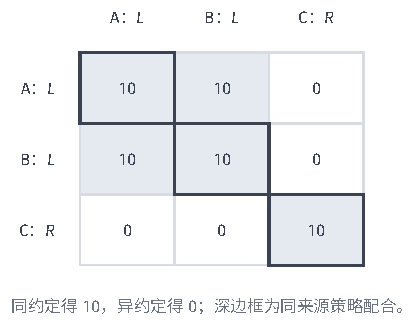
\includegraphics[width=69.977mm]{figures/07-reinforcement-learning/03-task-expansion-and-trustworthiness/tikz/rl-multi-agent-cross-play.pdf}
 \caption{两约定任务的交叉配合矩阵。各格给团队分，深边框标同来源对角；A、B使用$L$，C使用$R$，不兼容配对得0。数值由教学规则精确计算，并非实测成绩。}
 \label{fig:rl-multi-agent-cross-play}
\end{figure}

测试前应冻结训练群体、检查点选择和各伙伴的对局预算。可先对每个留出伙伴测零样本结果，再在预设$B\in\{0,5,20\}$等教学预算网格上测适应后表现；横轴记录实际交互，另列梯度步及记忆重置规则。若反复利用测试对手结果选检查点，它已被用于开发，需要重新留出，而非继续称为未见。

图中九格均匀平均为$50/9$，最差格为0，只平均三格对角却得到10。伙伴分布改变时，加权平均也改变，因此应同时报告矩阵、权重、平均和最坏已测表现。有限对局并未穷尽所有对手，最坏已测值仍不同于完整策略空间的最坏值，群体平均也不能提供不可利用性上界。

% Outline: 7.7.4
\subsection{固定样本、通信与计算预算下的效率评价}
\label{sec:rl-multi-agent-efficiency}

多智能体系统的资源消耗比单人复杂得多（一个联合环境步里其实包含$m$个参与者的动作），因此评价效率前必须统一计数口径，否则“更快”可能只是少算了某些通信或对手对局。

表\ref{tab:rl-multi-agent-resources}在每人$A$个离散动作、图边集$E_G$、消息维度$d_c$和消息传递轮数$L$的条件下，比较结构性操作成本。采样统一计联合步数$N$，达到某回报所需的$N$仍须实测。表中的计算阶数只说明列出的操作如何增长，不构成样本需求的推导。

\begin{table*}[htbp]
 \centering
 \begin{tabularx}{\linewidth}{@{}l >{\raggedright\arraybackslash}X >{\raggedright\arraybackslash}X >{\raggedright\arraybackslash}X >{\raggedright\arraybackslash}X@{}}
 \toprule
 结构 & 人数与动作计算 & 采样及训练权限 & 训练通信／存储 & 部署推理与通信\\
 \midrule
 联合价值枚举 & $m$人，$A^m$组合 & $N$联合步；集中输入 & 联合转移、动作与价值表或网络 & 若集中选动作，须具备实时集中权限\\
 VDN／QMIX & 局部比较$mA$次 & $N$联合步；QMIX混合器用状态 & 联合TD目标及训练反传 & $m$次局部网络；无必需执行消息\\
 集中评论家、局部行动者 & 每人一次动作输出 & $N$联合步；声明评论家状态／动作输入 & 回放或近期轨迹及集中特征 & 局部推理；共享参数不等于共享观测\\
 图消息策略 & $m$节点、$|E_G|$条边 & $N$联合步；合法训练图 & 消息及历史按实现记录 & $L|E_G|d_c$量级消息元素，$L$轮同步\\
 PSRO群体 & 双方各$K$个库策略 & 响应样本加收益表对局；权限继承响应器 & $K^2$表项及多个检查点 & 回合抽索引再执行；未必同时运行全部网络\\
 \bottomrule
 \end{tabularx}
 \caption{训练与部署的结构性资源需求。所列复杂度只针对对应操作，不等于总运行时间，也不证明达到某一回报的样本复杂度。}
 \label{tab:rl-multi-agent-resources}
\end{table*}

消息拓扑对成本的影响可由图\ref{fig:rl-multi-agent-scaling}的串行模型说明。设每条有向边处理一条消息耗时0.01毫秒，全部节点动作计算耗时$0.05m$毫秒。全连接具有$m(m-1)$条边；局部图在此按每人恰向$\min(4,m-1)$个出邻居发消息计算，共有$m\min(4,m-1)$条边，这是“最多4个”的满额情形。按节点和边逐项相加，得到
\[
 \begin{aligned}
 T_{\text{全连}}(m)&=0.05m+0.01m(m-1),\\
 T_{\text{局部}}(m)&=0.05m+0.01m\min(4,m-1).
 \end{aligned}
\]
代入$m=20$，两种解析时延分别为4.8和1.8毫秒。它们只成立于所给串行模型，并非硬件测试；真实设备的并行、拥塞及同步开销都可能改变结果。

\begin{figure}[htbp]
 \centering
 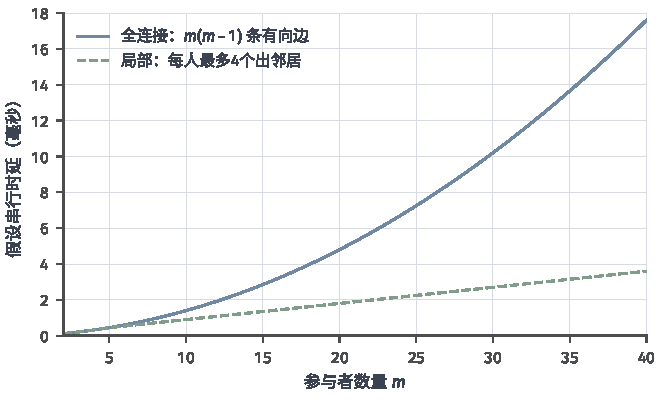
\includegraphics[width=112.000mm]{figures/07-reinforcement-learning/03-task-expansion-and-trustworthiness/matplotlib/rl-multi-agent-scaling.pdf}
 \caption{串行消息模型中的跨规模成本。全连接与最多4邻居的局部交互采用相同节点和边成本；稀疏图降低消息量，但可能同时删去任务需要的远端参与者状态或消息。}
 \label{fig:rl-multi-agent-scaling}
\end{figure}

资源比较应保留这些取舍：复用同一结构的参数可减少模型存储，却仍须为不同历史计算动作；集中状态与联合历史可帮助估计，却增加训练传输；通信可改善协调，却增加收发与同步开销，是否增加总时延还取决于并行实现。跨规模测试还须控制拥挤度、瓶颈容量和观测、历史与消息读取权限，否则成本增长与任务难度变化混在一起，难以解释曲线。

% Outline: 7.7.5
\subsection{行为评价与复现所需的协议信息}
\label{sec:rl-multi-agent-protocol}

多智能体结果尤其难复现，因为即使恢复了网络参数和随机种子，只要训练时的对手配对、各人行动前可读取的观测、历史与消息等交互条件没还原，结果就可能完全不同。因此复现不仅要恢复参数和随机种子，还须恢复参与者配对与交互权限。

\begin{table*}[htbp]
 \centering
 \small
 \begin{tabularx}{\linewidth}{@{}l >{\raggedright\arraybackslash}X >{\raggedright\arraybackslash}X@{}}
 \toprule
 协议项 & 必须记录的内容 & 主要影响环节\\
 \midrule
 参数共享与身份 & 共享哪些模块；编号、角色编码及重排规则 & 参数梯度汇总与执行约定\\
 集中状态与屏蔽 & 评论家输入；合法动作掩码由谁提供 & 训练权限及执行动作分布\\
 死亡、退出与终止 & 占位观测、动作、损失屏蔽；全局或个体终止 & 价值目标、占用统计和人数\\
 回放与版本 & 来源检查点、窗口、概率字段、校正与采样权重 & 联合经验的目标匹配\\
 对手与伙伴抽样 & 库版本、保留及淘汰、抽样概率、是否在线学习 & 训练和评价的参与者分布\\
 通信 & 发送／接收权限、载荷、时序、延迟、带宽 & 部署可行性与成本\\
 回报与评价 & 奖励尺度、塑形、回合上限、偏离类及间隙约定 & 行为标准和比较口径\\
 \bottomrule
 \end{tabularx}
 \caption{复现多智能体结果所需的最小协议。各项可能改变策略、环境或验证对象，因此超参数表之外还需保存这些交互条件。}
 \label{tab:rl-multi-agent-protocol}
\end{table*}

还应保存伙伴与对手的生成流程、策略库和检查点标识、用于检查点选择的验证参与者，以及各组合的评估场数。训练初始化、环境随机性和伙伴抽样宜采用可追踪的独立随机源。若5次独立训练各评价1000局，独立训练运行仍只有5个，不能把5000场对局当作5000次独立训练。同一检查点或同一适应链上的对局可能相关，区间估计应保留训练运行与伙伴层级。

第三方对手、外部游戏版本或消息服务若无法恢复，应列明限制。所存材料可以支持在这些伙伴与接口下重现结果，未必支持对所有未知参与者成立。只有声明、协议和证据对应同一对象，评价范围才清楚。

% Outline: 7.8
\section{本章小结}
\label{sec:rl-multi-agent-summary}

同一个通道动作会随对方行为产生不同后果，因而多智能体求解要先明确收益、观测与消息权限及参与者变化。收益关系决定采用团队最优、极小极大还是单方偏离标准，社会分配目标须另行规定；观测与消息读取权限限定策略可依赖的历史字段，集中训练不能扩大部署可见范围；其他人继续学习时，边缘化后的行为后果也可能不再平稳。

经验采集须记录联合动作、消息与参与者来源，并检查目标的联合支持；边缘动作都出现过，仍可能无法识别所需的配合效果。在此基础上，联合价值、个体替代、局部组合、伙伴类型和响应模型保留不同依赖，可共同提供更新所需的估计。价值或梯度计算还须与相互适应和群体组织配合。局部贪心一致不等于整表可表示，单次改进不等于共同动态稳定，库内近似响应也不能认证完整博弈不可利用。

验证时，外部与内部遗憾分别约束粗相关和相关经验分布；利用零和抵消才能进一步控制适当平均策略的鞍点间隙，当前策略却未必收敛。训练对手收益、留出伙伴协调、跨规模表现与资源成本也须分别报告。使用伙伴反馈更新记忆或类型已属适应，即使参数不变，也不能记为零样本。明确行为标准、参与者范围、可读观测与消息和交互预算之后，结果才有可解释的边界。第\ref{chap:rl-trustworthy}章将转向风险、扰动和安全约束这一类行为要求；性能证据并不自动成为安全保证，多方任务仍需保留本章的联合行为、局部观测与消息时序条件。
